\documentclass[a4paper]{article}
\usepackage[utf8]{inputenc}
\usepackage[english]{babel}
\usepackage[T1]{fontenc}
\usepackage{lmodern}
\usepackage{fullpage}
\usepackage{amsmath}
\usepackage{graphicx}
\usepackage{framed}
\usepackage{listings}
\usepackage{placeins}
\usepackage{subcaption}
\usepackage{array}
\usepackage[justification=centering]{caption}

\author{Théotime Grohens}
\title{Introduction to Computer Vision: \\ Assignment 2: Canny Edge Detector}

\begin{document}

\maketitle

\subsection*{Question 1}

Here are the original images the edges of which we are going to compute in the assignment :

\begin{figure}[h]
\centering

\begin{subfigure}{0.49\textwidth}
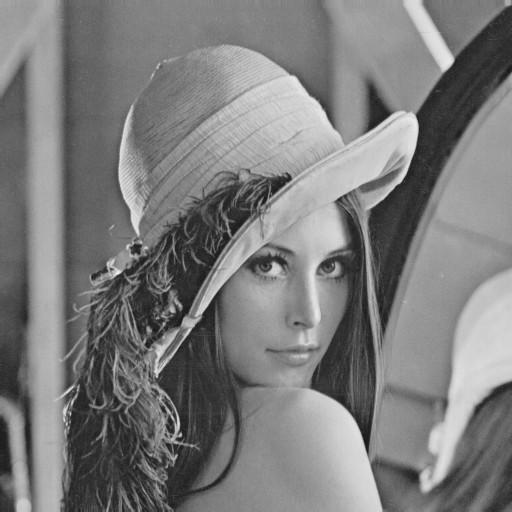
\includegraphics[width=\textwidth]{lena.jpg}
\caption{Lena.}
\end{subfigure} 
\begin{subfigure}{0.49\textwidth}

\includegraphics[width=\textwidth]{cat.jpg}
\caption{A cat wrapped in kraft paper.}
\end{subfigure}
\end{figure}

\FloatBarrier

\subsection*{Question 2}

In this section, we show the result of applying an edge mask using a simple threshold on the image magnitude matrices.

\begin{figure}[h]

\begin{subfigure}{0.33\textwidth}
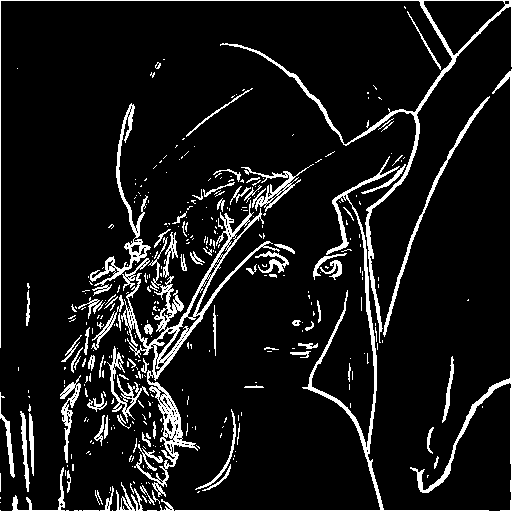
\includegraphics[width=\textwidth]{img/sigma1/lenast.png}
\end{subfigure}
\begin{subfigure}{0.33\textwidth}
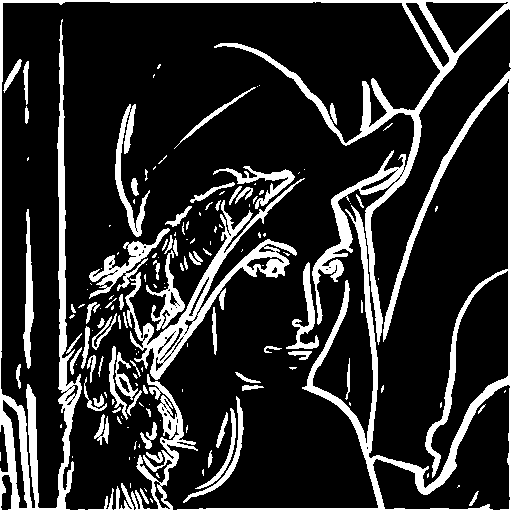
\includegraphics[width=\textwidth]{img/sigma2/lenast.png}
\end{subfigure}
\begin{subfigure}{0.33\textwidth}
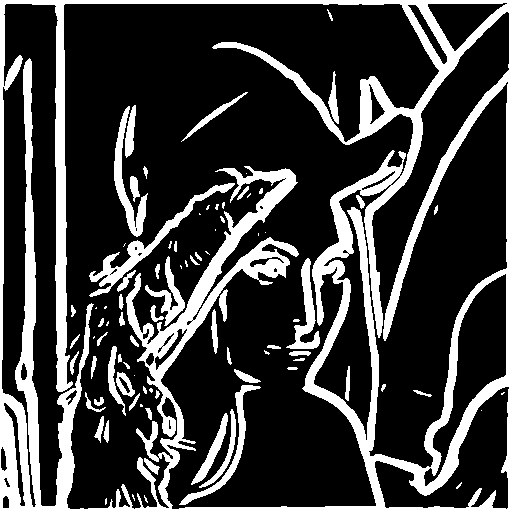
\includegraphics[width=\textwidth]{img/sigma3/lenast.png}
\end{subfigure}

\begin{subfigure}{0.33\textwidth}
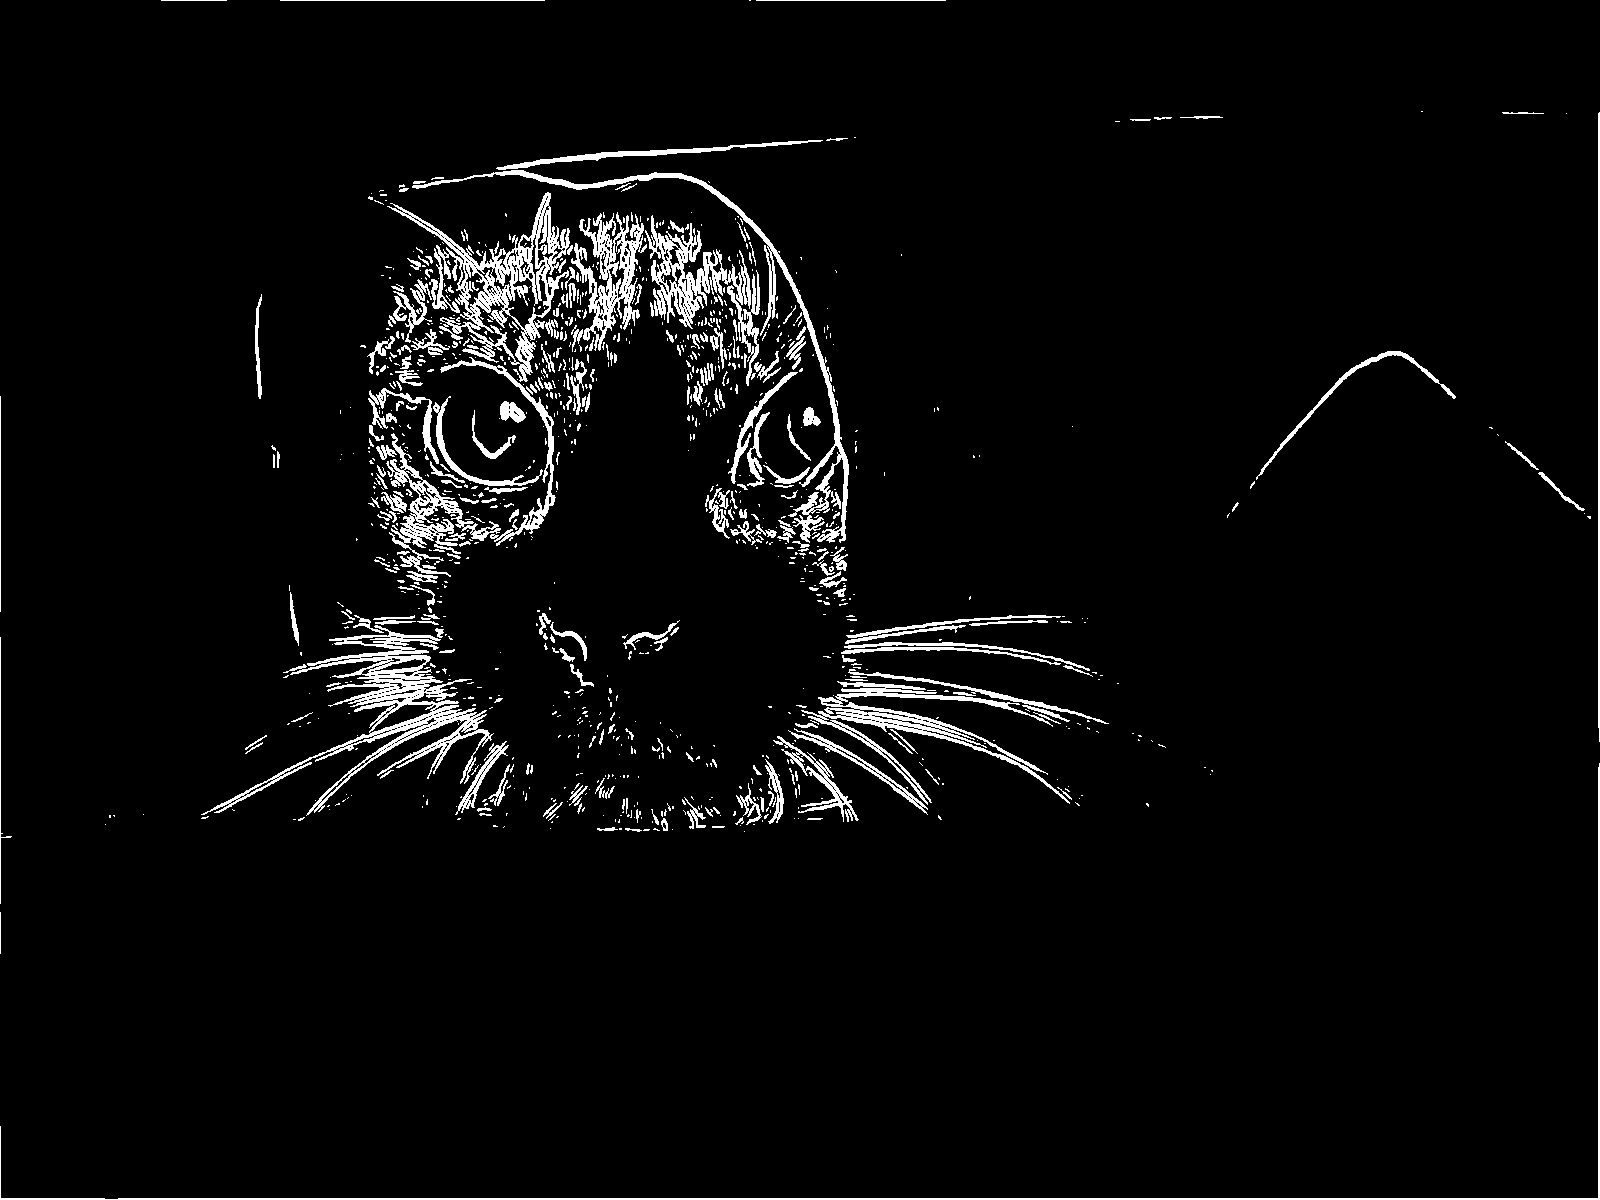
\includegraphics[width=\textwidth]{img/sigma1/catst.png}
\end{subfigure}
\begin{subfigure}{0.33\textwidth}
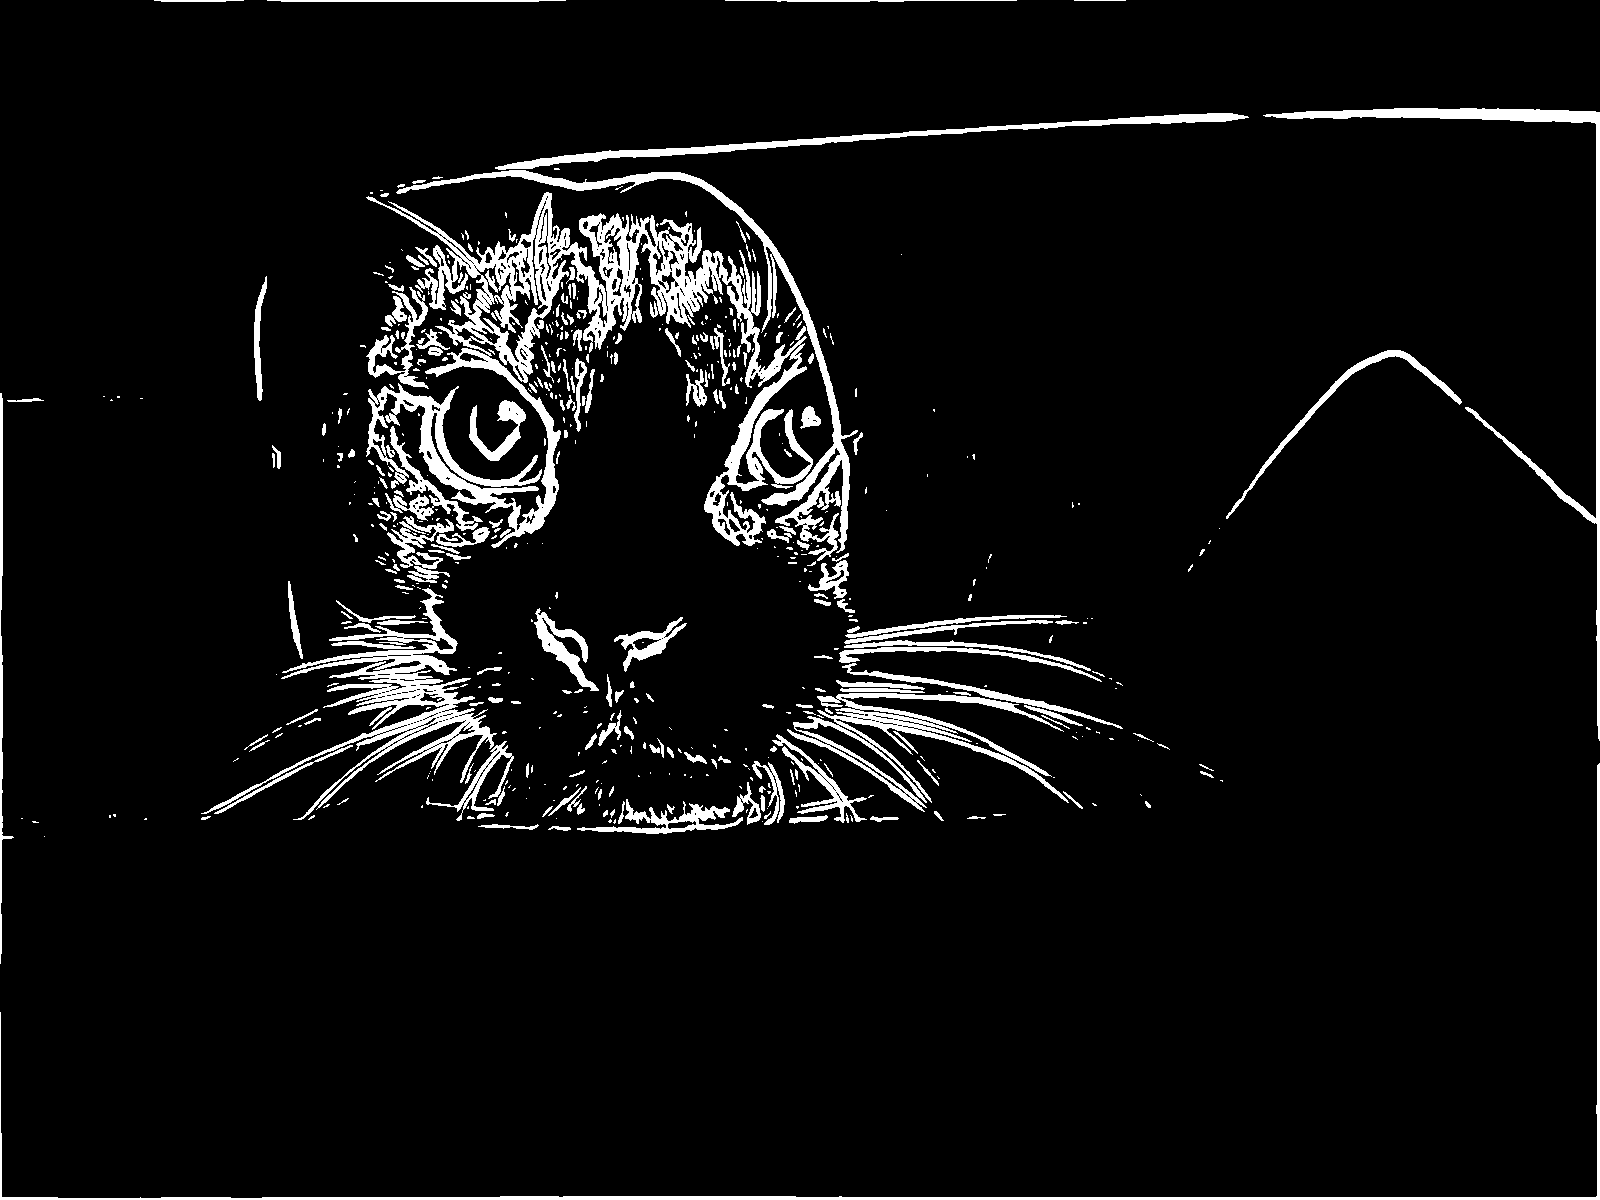
\includegraphics[width=\textwidth]{img/sigma2/catst.png}
\end{subfigure}
\begin{subfigure}{0.33\textwidth}
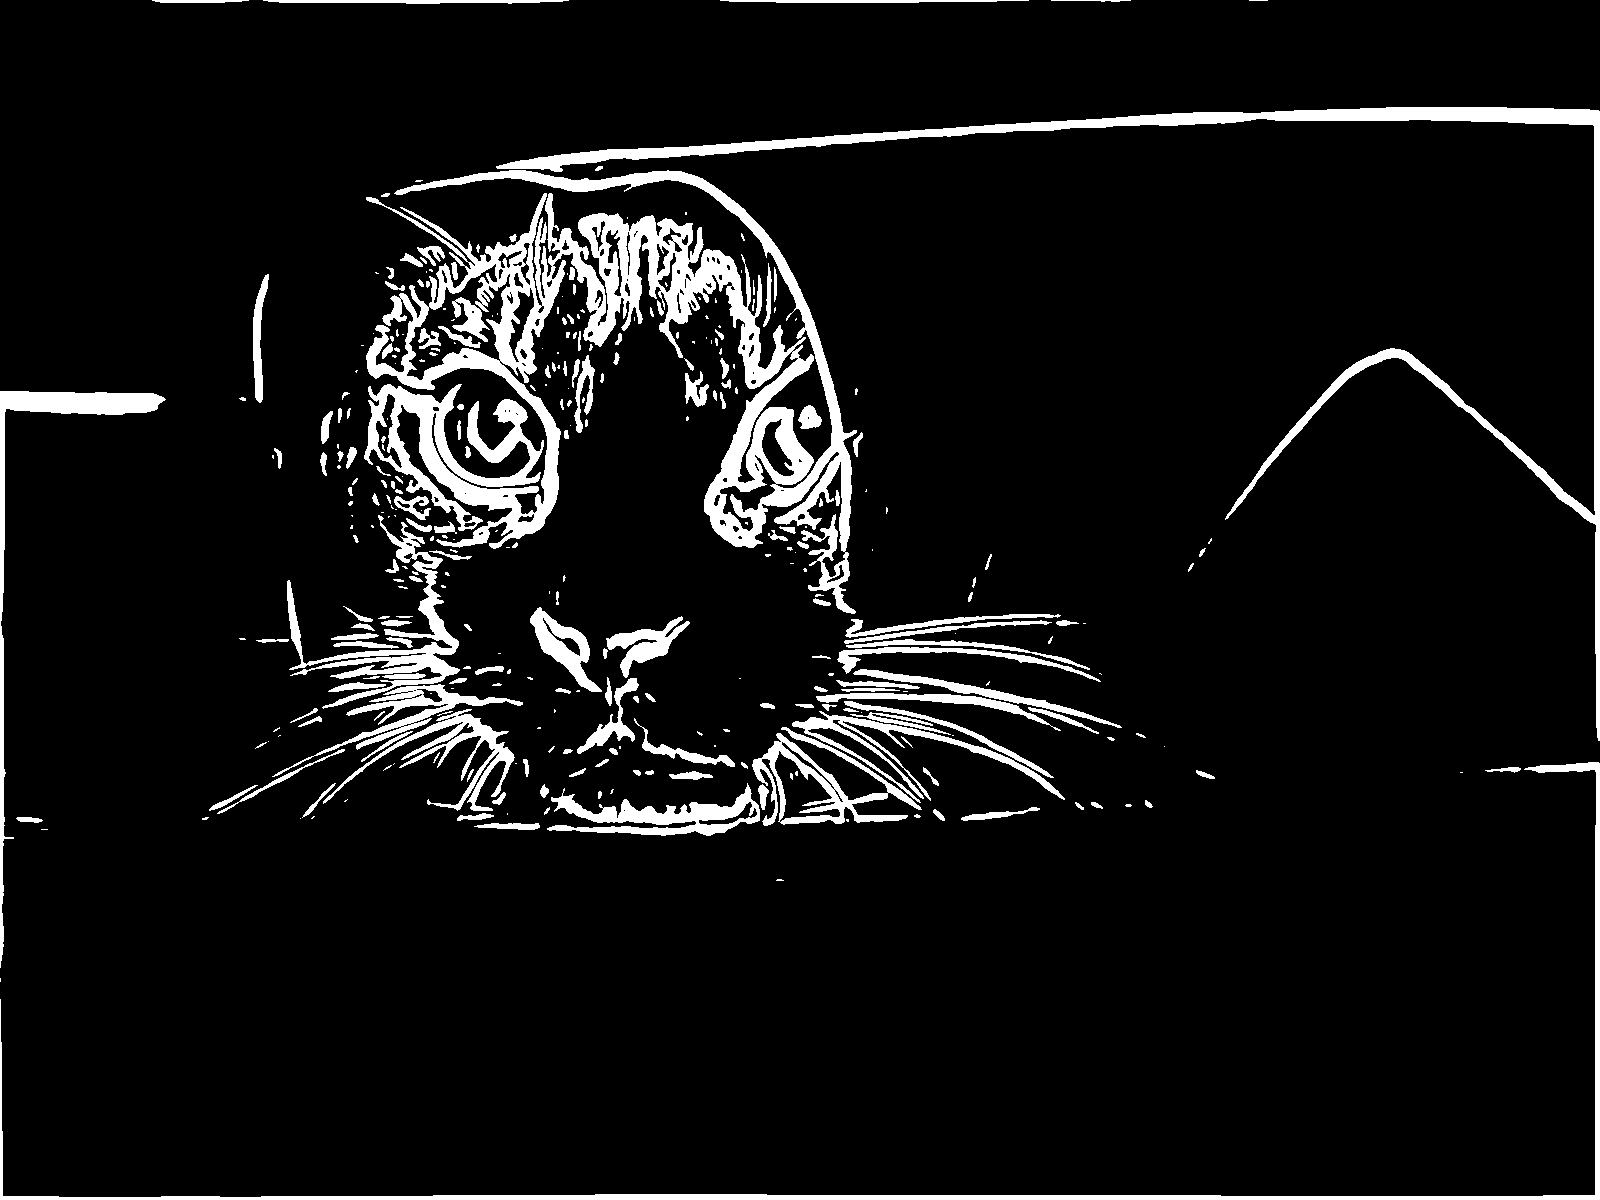
\includegraphics[width=\textwidth]{img/sigma3/catst.png}
\end{subfigure}

\caption{Simple edge mask, with $\sigma $ = 1, 2 or 3, and a threshold value of 0.15.}

\end{figure}

These images show that, as $\sigma$ increases, the edges get blurrier.
This also allows us to get rid of well-defined but less important edges, which get blurred away: for example, Lena's hair becomes less detailed as $\sigma$ increases.
On the contrary, more important but blurrier edges appear better with higher values of $\sigma$: for example, the cat's nose and eyes stand out better as $\sigma$ increases.

The value of the threshold is 0.15, which means that pixels having at least 15\% of the maximum magnitude appear. Higher thresholds would make us lose detail, and lower thresholds would add too many points to the mask.

\FloatBarrier

\subsection*{Question 3}

In this section, we apply non-maximum suppression to the image magnitude matrices.
This allows us to only keep points that are local maxima of magnitude in the direction of the gradient (which is perpendicular to the edge we're looking for).
In a sense, this should allow us to only keep the most important points of edges, making all of them 1 pixel wide.

Once edges are well-enough defined, as we see in the pictures, we can get rid of the least important ones with a simple thresholding.
The values of $\sigma$ and the threshold are the same as in the former question.

\begin{figure}[h]

\begin{subfigure}{0.33\textwidth}
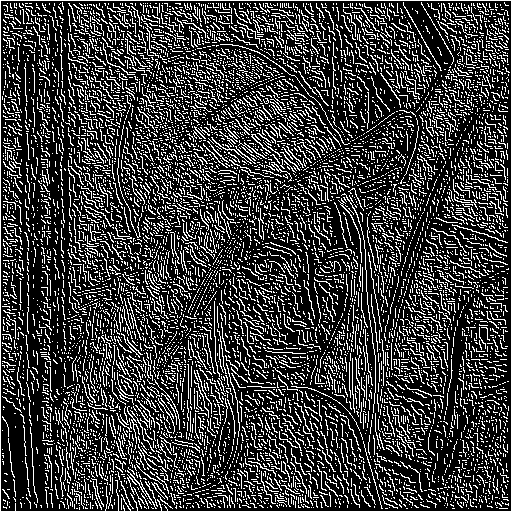
\includegraphics[width=\textwidth]{img/sigma1/lenanon.png}
\end{subfigure}
\begin{subfigure}{0.33\textwidth}
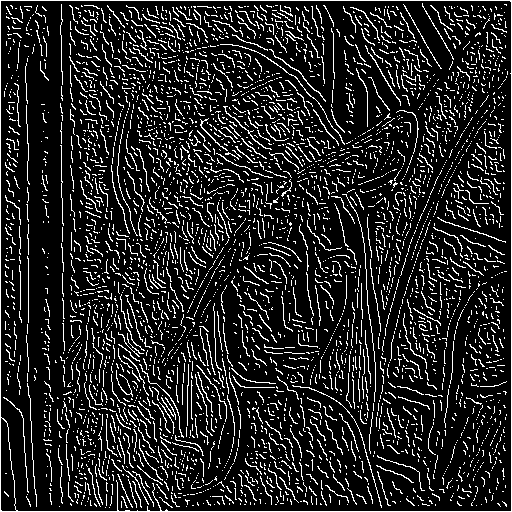
\includegraphics[width=\textwidth]{img/sigma2/lenanon.png}
\end{subfigure}
\begin{subfigure}{0.33\textwidth}
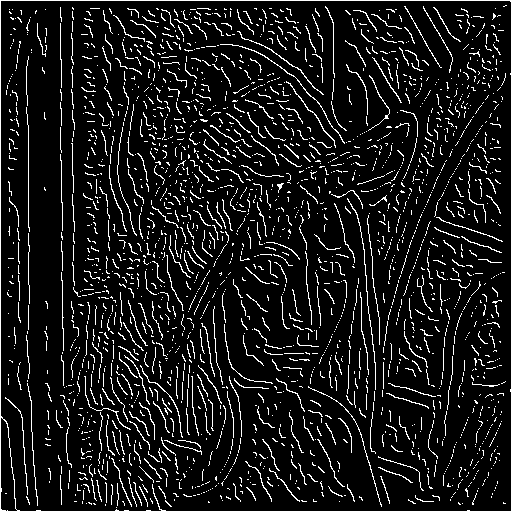
\includegraphics[width=\textwidth]{img/sigma3/lenanon.png}
\end{subfigure}

\begin{subfigure}{0.33\textwidth}
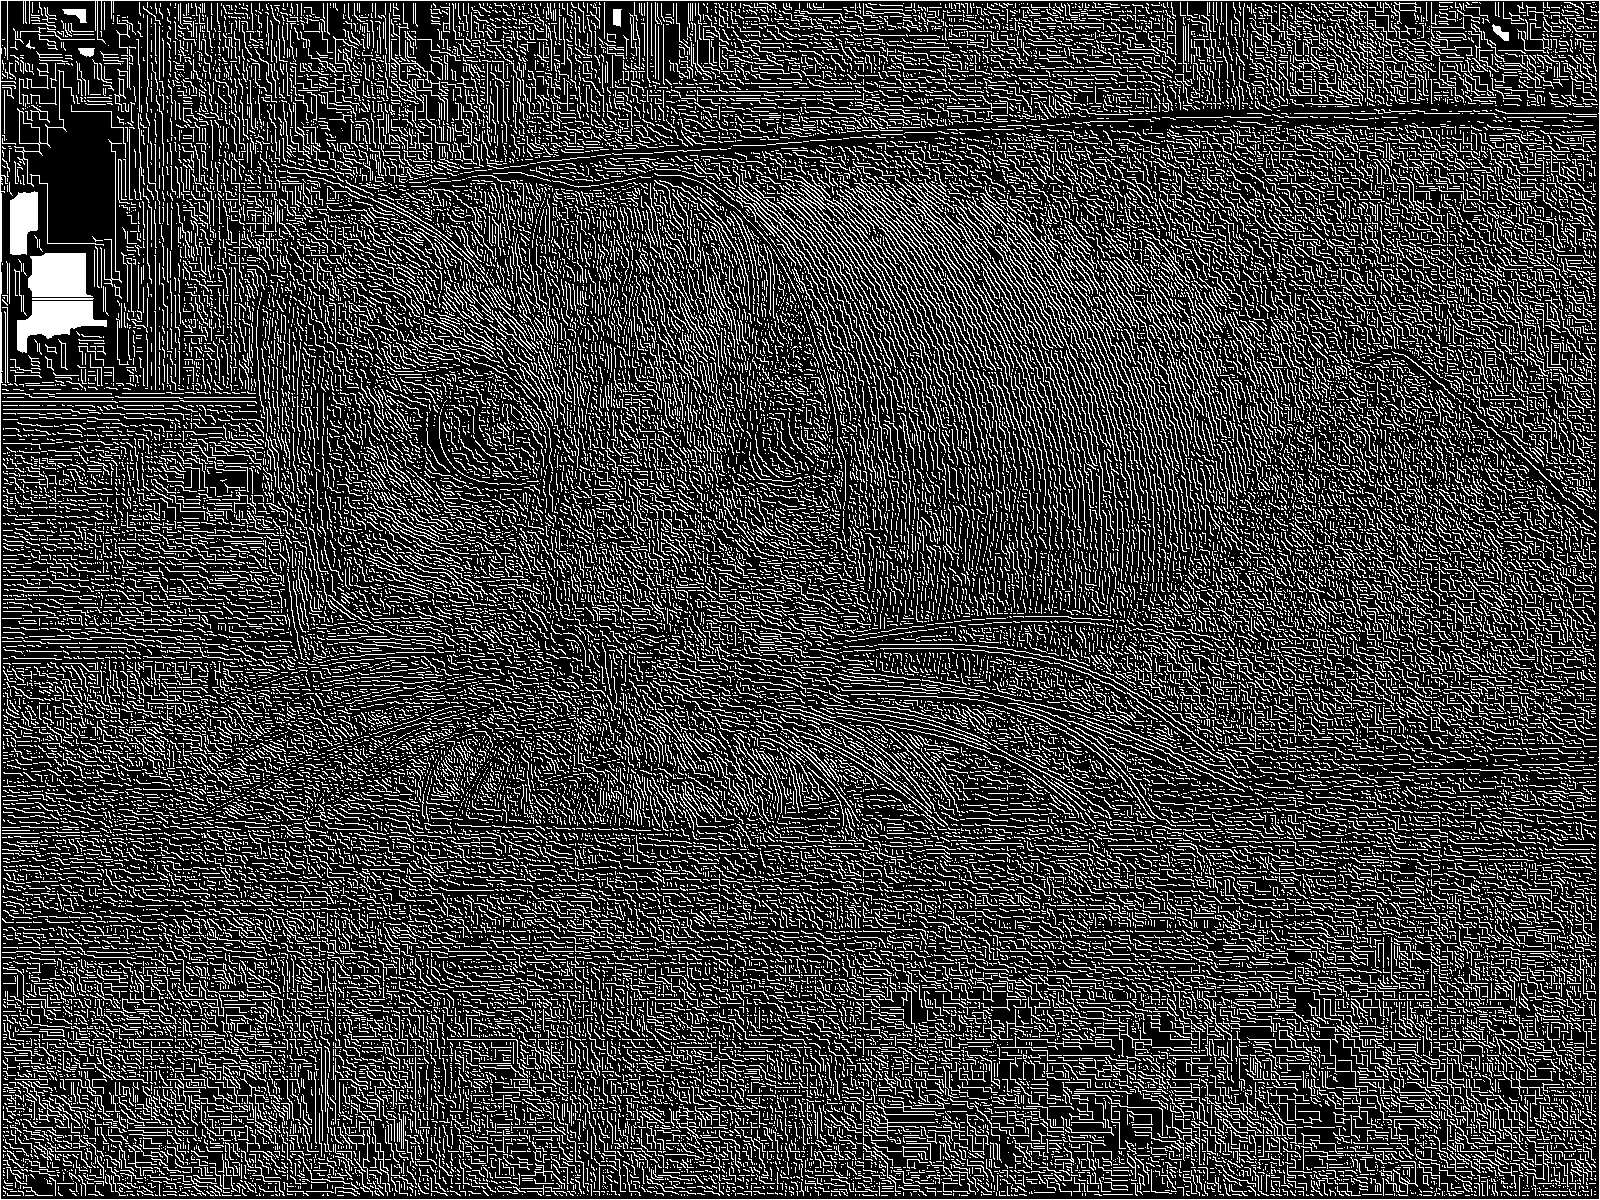
\includegraphics[width=\textwidth]{img/sigma1/catnon.png}
\end{subfigure}
\begin{subfigure}{0.33\textwidth}
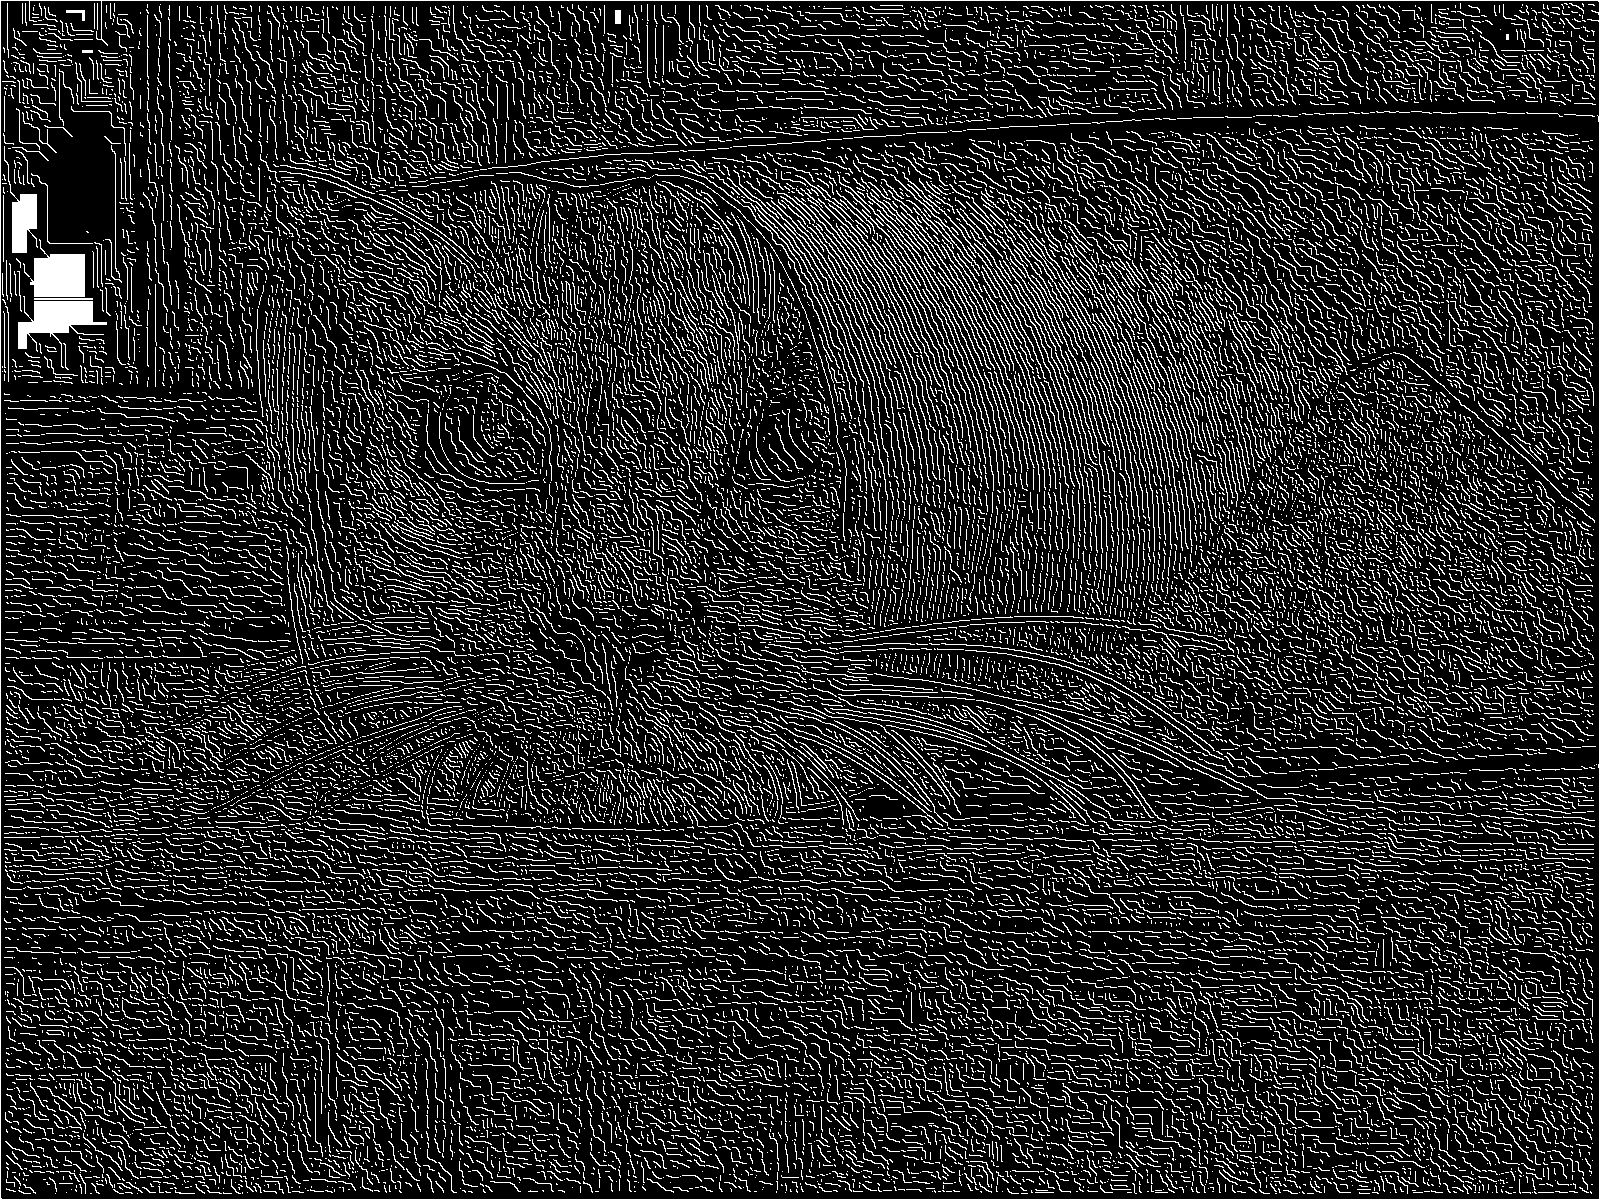
\includegraphics[width=\textwidth]{img/sigma2/catnon.png}
\end{subfigure}
\begin{subfigure}{0.33\textwidth}
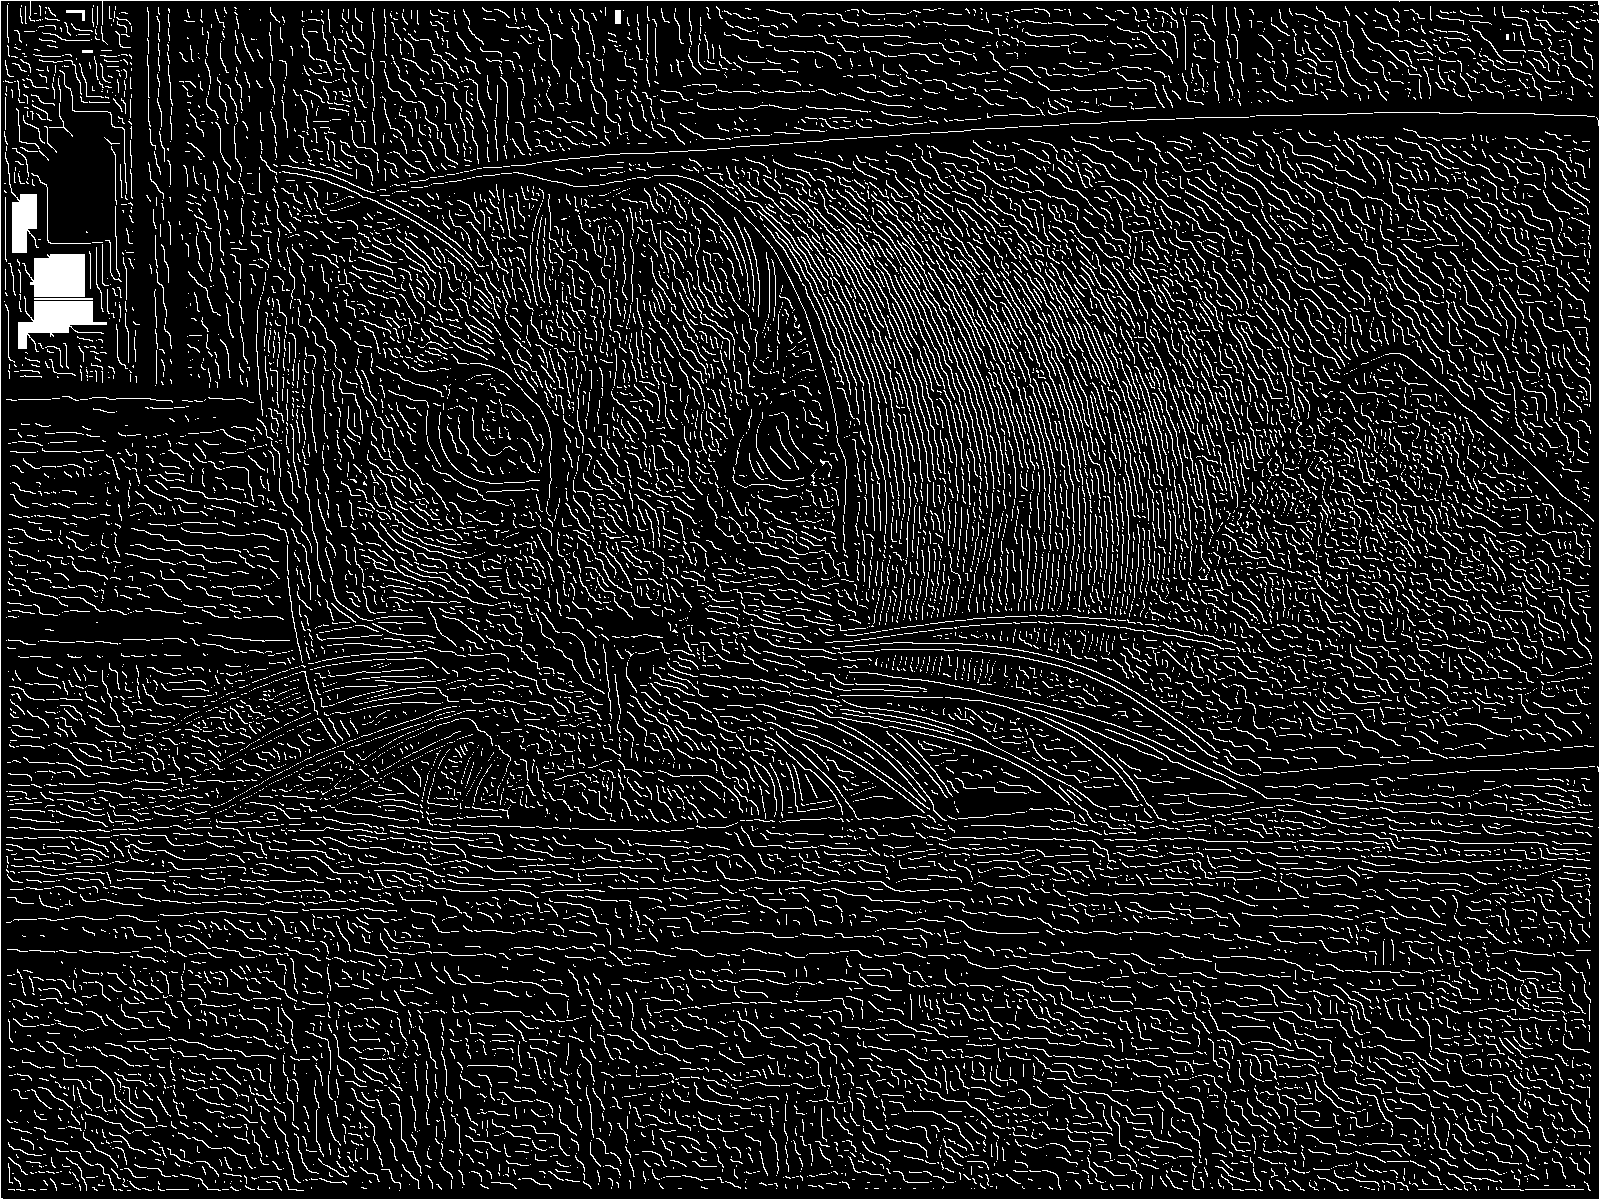
\includegraphics[width=\textwidth]{img/sigma3/catnon.png}
\end{subfigure}

\caption{Non-maximum suppression, without thresholding. $\sigma$ = 1, 2 and 3.}

\end{figure}

\FloatBarrier

For lower values of $\sigma$, which add less blur to the original image, we get a lot of spurious edges (which will however disappear once we apply thresholding).
When we blur the image more, nearby edges blend, and since the non-maximum suppression only keeps 1 pixel-wide edges, we see a clear reduction in the number of edges.

\begin{figure}[h]

\begin{subfigure}{0.33\textwidth}
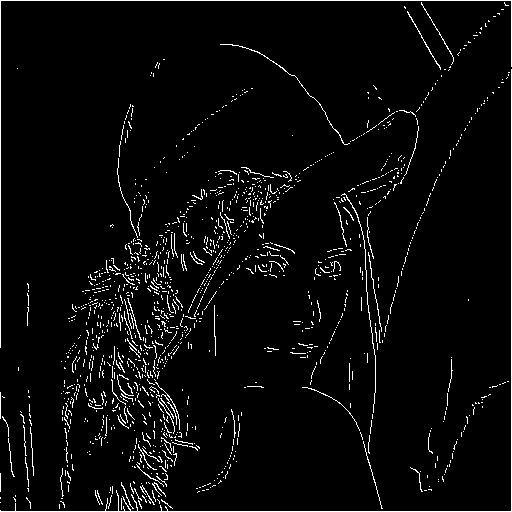
\includegraphics[width=\textwidth]{img/sigma1/lenanont.png}
\end{subfigure}
\begin{subfigure}{0.33\textwidth}
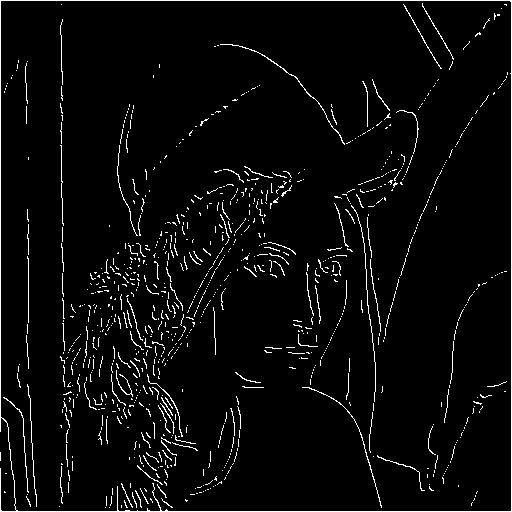
\includegraphics[width=\textwidth]{img/sigma2/lenanont.png}
\end{subfigure}
\begin{subfigure}{0.33\textwidth}
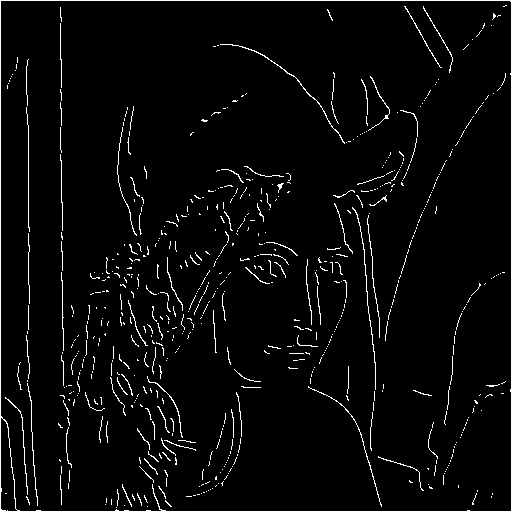
\includegraphics[width=\textwidth]{img/sigma3/lenanont.png}
\end{subfigure}

\begin{subfigure}{0.33\textwidth}
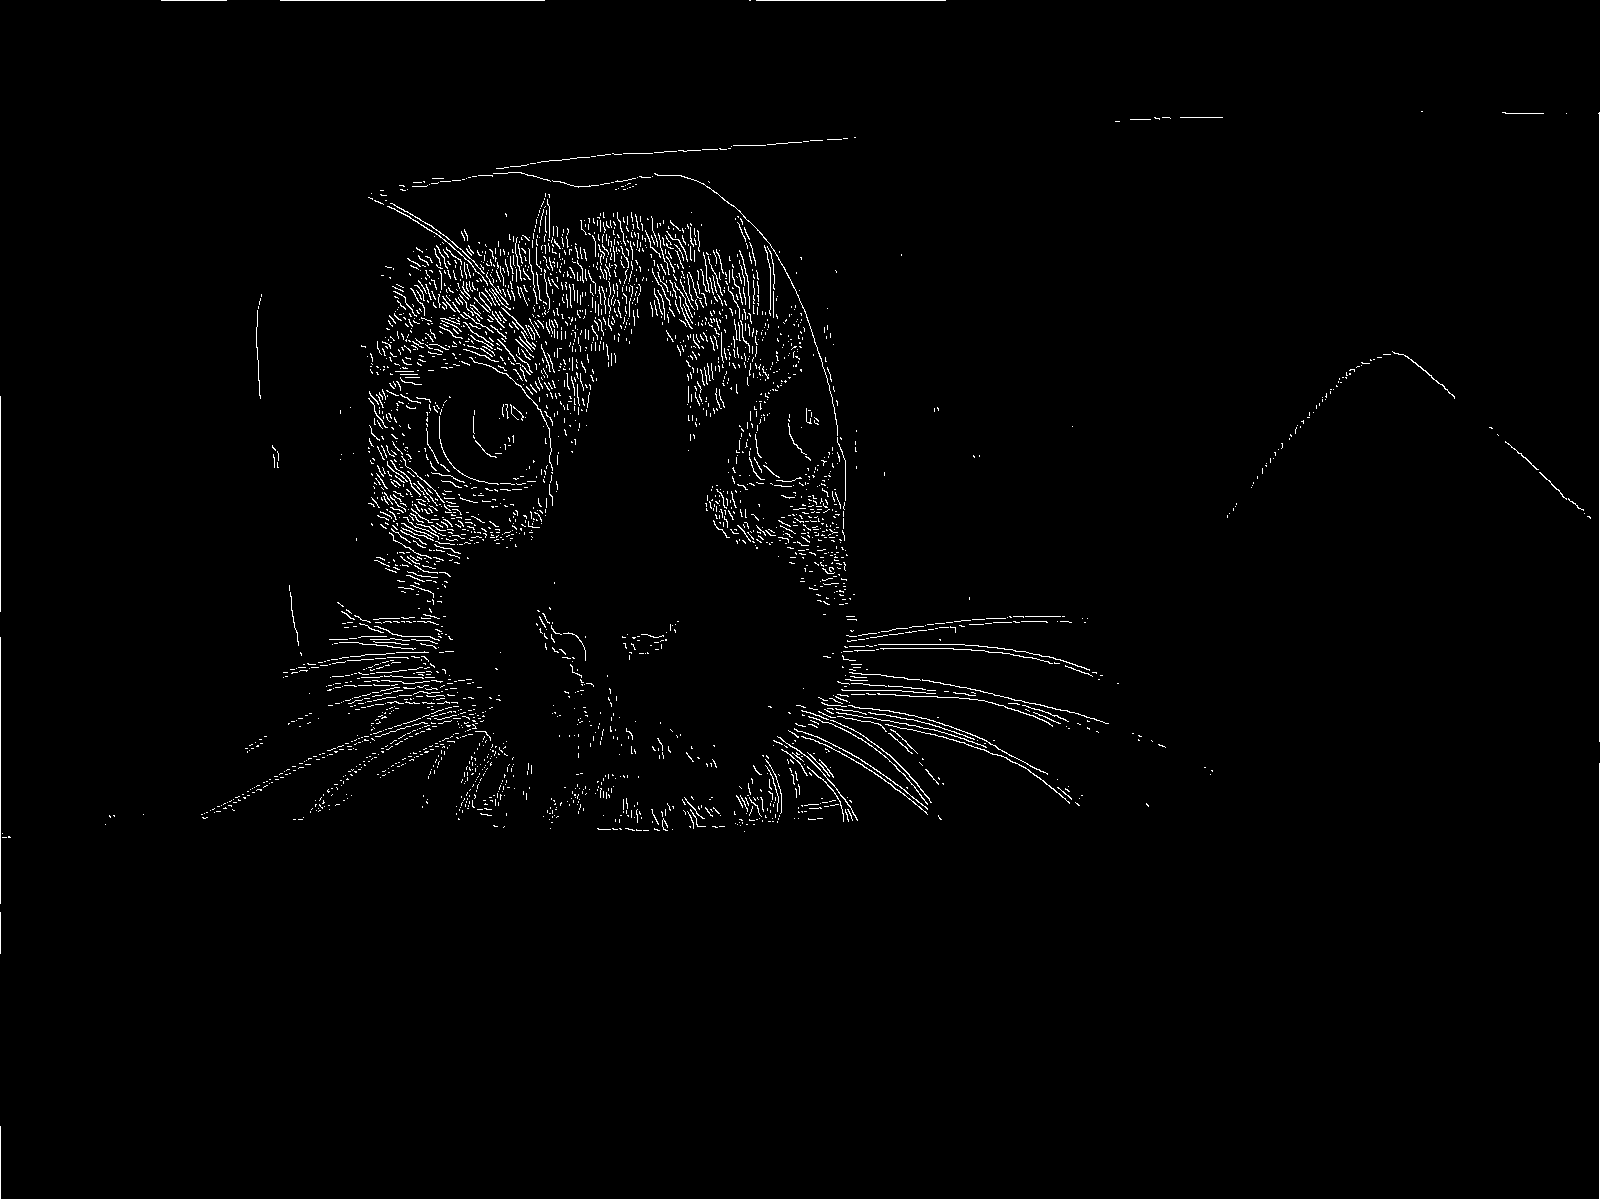
\includegraphics[width=\textwidth]{img/sigma1/catnont.png}
\end{subfigure}
\begin{subfigure}{0.33\textwidth}
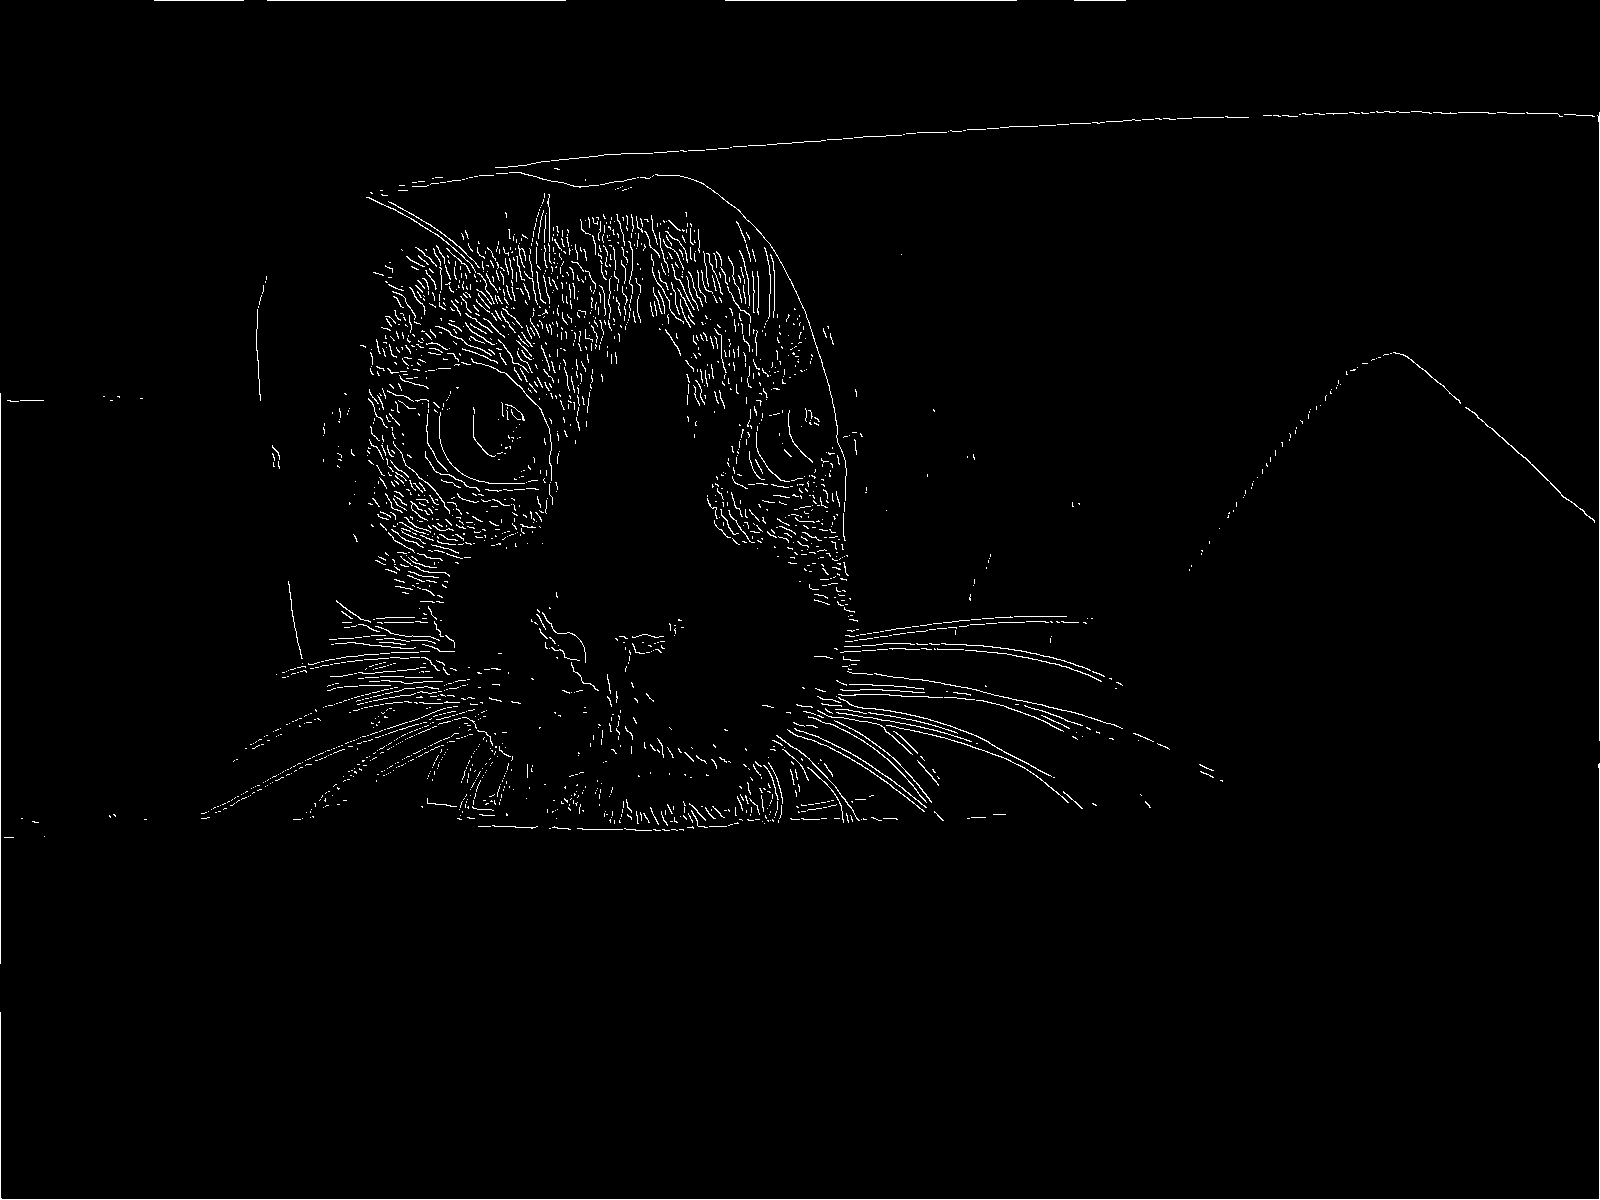
\includegraphics[width=\textwidth]{img/sigma2/catnont.png}
\end{subfigure}
\begin{subfigure}{0.33\textwidth}
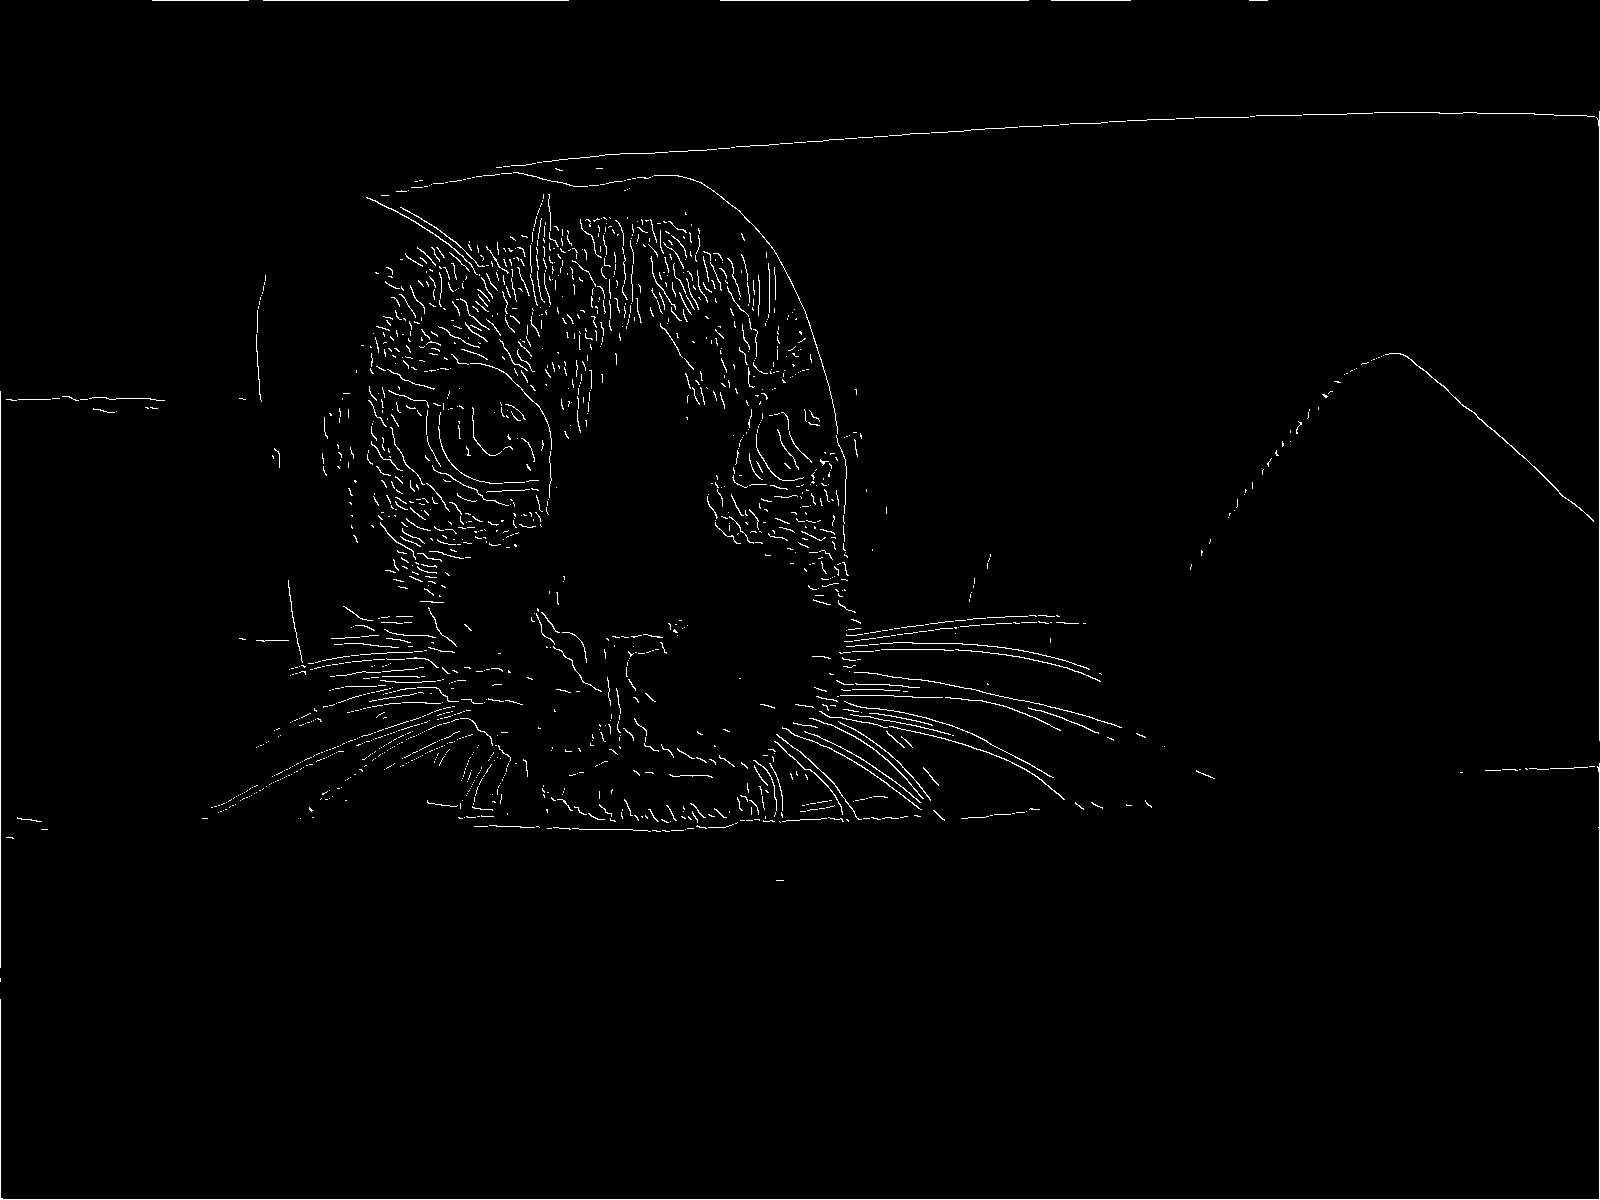
\includegraphics[width=\textwidth]{img/sigma3/catnont.png}
\end{subfigure}

\caption{Non-maximum suppression, with thresholding. $\sigma$ = 1, 2 and 3.}

\end{figure}

With the thresholding, only the most important edges are kept.
We can see that this reflects much more clearly our intuitive vision of what the edges should be in the original images.
As before, lower values of $\sigma$ offer us more detail on well-defined edges, but lose track of blurrier ones: we can see Lena's nose appear more clearly as $\sigma$ increases, but we lose precision in her hair.
The mouth and nose of the cat also appears more clearly for higher values of $\sigma$, but his eyes get a little blurrier.

\FloatBarrier

\subsection*{Question 4}

Hysteresis thresholding is a technique that allows us to keep a little more pixels qualified as edges, while not adding too many spurious ones.
It is based on the intuition that, even if a certain pixel (which is a local maximum of magnitude in the direction of the gradient) is under the threshold that we chose, it might still be part of an actual edge if it is the neighbour of a pixel that is part of one.

In order to do that, we first keep pixels over our magnitude threshold, and then iteratively add edges that are over a lower threshold, but still connected to edge pixels.
The results of this technique are shown in the pictures: we do keep more pixels than with the simple threshold of the former question, but they are still part of existing edge lines and do not add any new ones.

Hysteresis thresholding allows us to get some of the lines of the kraft paper in the cat picture, for example, which do not appear with the other techniques.

\begin{figure}[h]

\begin{subfigure}{0.33\textwidth}
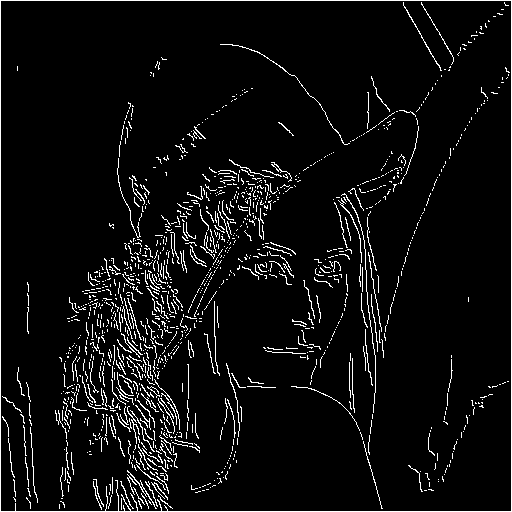
\includegraphics[width=\textwidth]{img/sigma1/lenahys.png}
\end{subfigure}
\begin{subfigure}{0.33\textwidth}
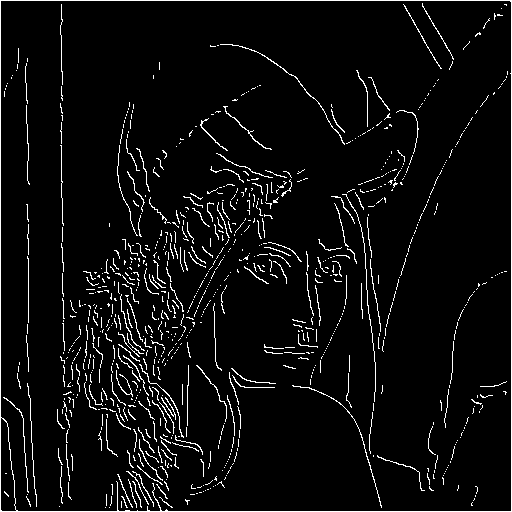
\includegraphics[width=\textwidth]{img/sigma2/lenahys.png}
\end{subfigure}
\begin{subfigure}{0.33\textwidth}
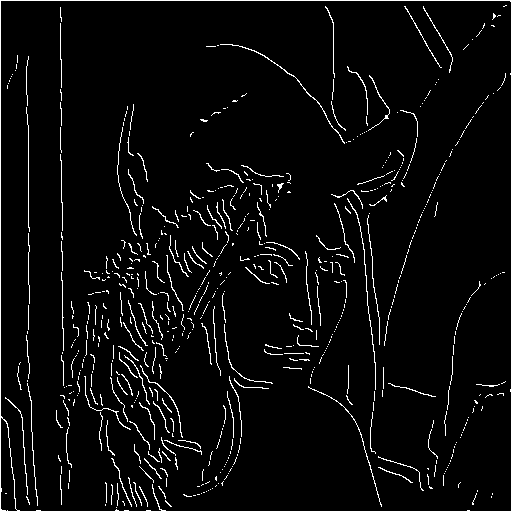
\includegraphics[width=\textwidth]{img/sigma3/lenahys.png}
\end{subfigure}

\begin{subfigure}{0.33\textwidth}
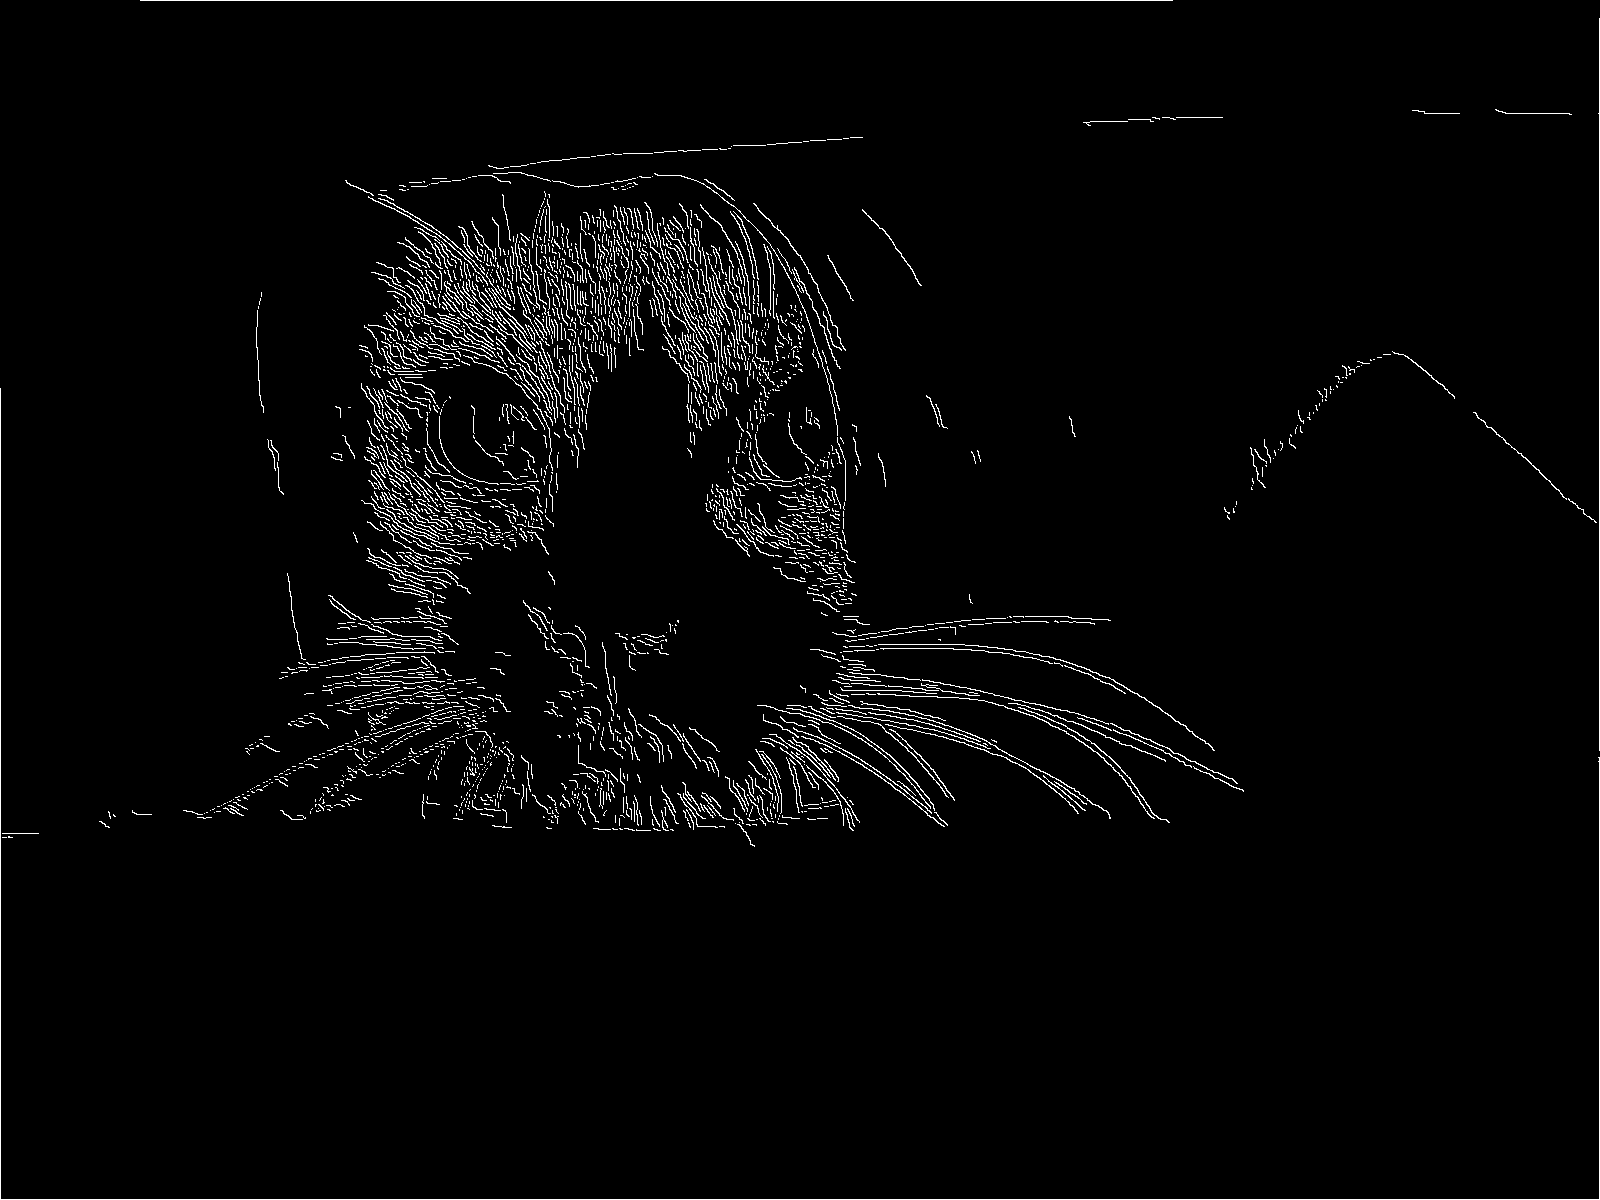
\includegraphics[width=\textwidth]{img/sigma1/cathys.png}
\end{subfigure}
\begin{subfigure}{0.33\textwidth}
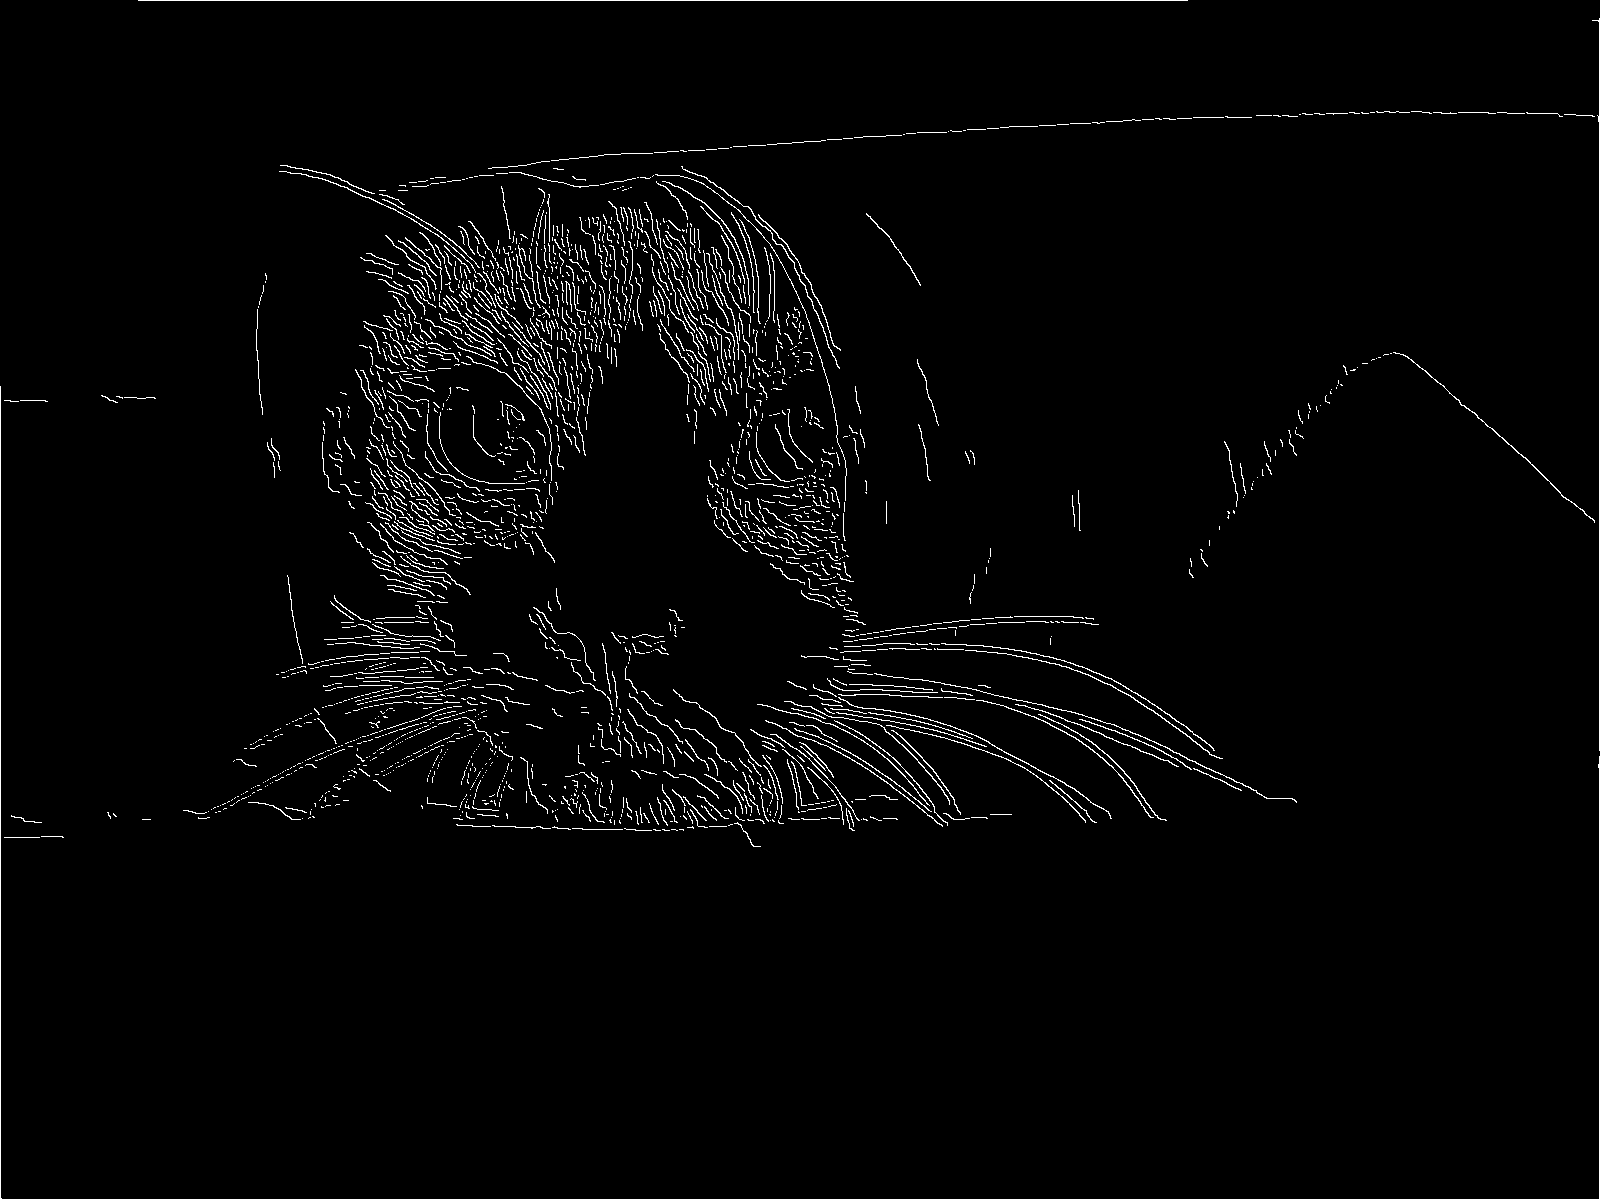
\includegraphics[width=\textwidth]{img/sigma2/cathys.png}
\end{subfigure}
\begin{subfigure}{0.33\textwidth}
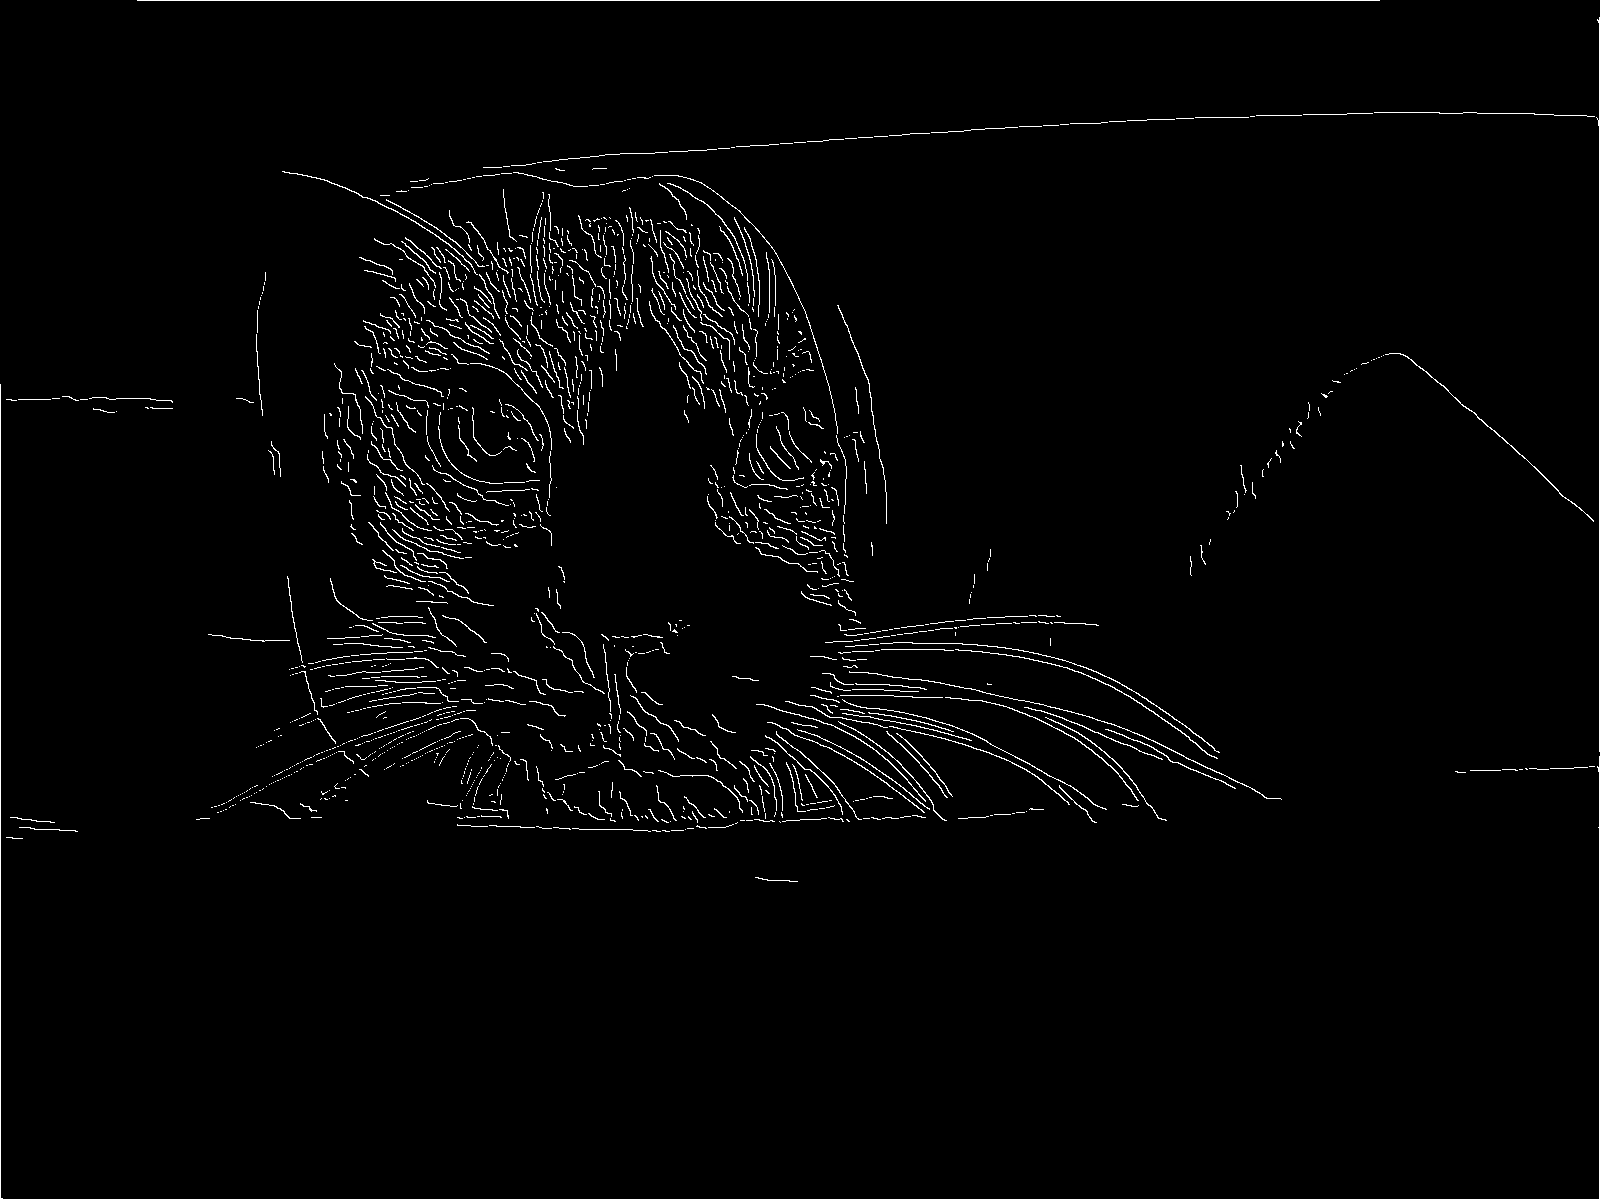
\includegraphics[width=\textwidth]{img/sigma3/cathys.png}
\end{subfigure}

\caption{Hysteresis thresholding. $\sigma$ = 1, 2 and 3; the high and low thresholds are 0.15 and 0.025.}

\end{figure}

\FloatBarrier

We ran the hysteresis thresholding again with a low threshold value of 0, which means that we kept all local magnitude maximal that were transitively connected to a local magnitude maximum over the high threshold.
This allows us to, in a sense, run the edges all the way until the end.
However, as we can see in the pictures, this does not add many new pixels to the images.

This tells us that the high threshold value is really the significant parameter here, which we can interpret by saying that it rules over which edges are real and which ones are spurious; then, the hysteresis thresholding only adds a little precision but does not make new decisions about adding new edges to be detected.

In both hysteresis cases, if we had chosen higher values for the high threshold, we would have had more false negatives (edges that we think are real but are not chosen by the algorithm).
Conversely, if we had chosen a lower value, we would have had more false positives (spurious edges that were chosen by the algorithm).
This is clearly shown by the extreme case of the high threshold being 0, that we can see in the non-maximum suppression without thresholding of question 3.

\begin{figure}[h]

\begin{subfigure}{0.33\textwidth}
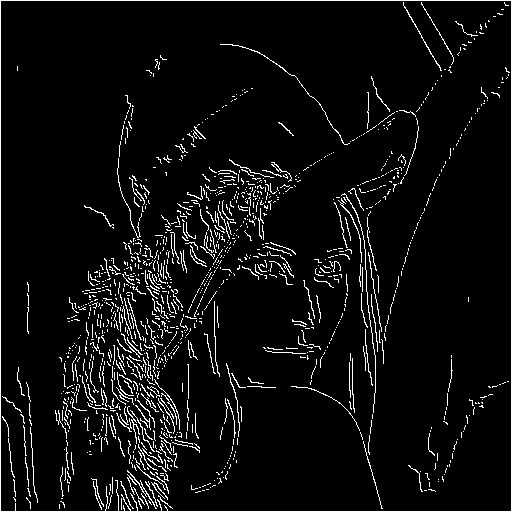
\includegraphics[width=\textwidth]{img/sigma1/lenahys0.png}
\end{subfigure}
\begin{subfigure}{0.33\textwidth}
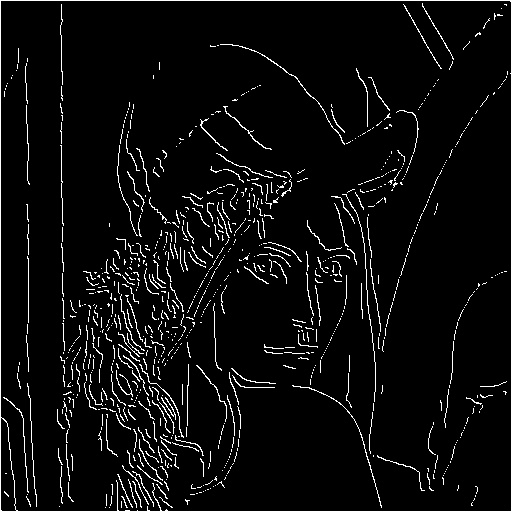
\includegraphics[width=\textwidth]{img/sigma2/lenahys0.png}
\end{subfigure}
\begin{subfigure}{0.33\textwidth}
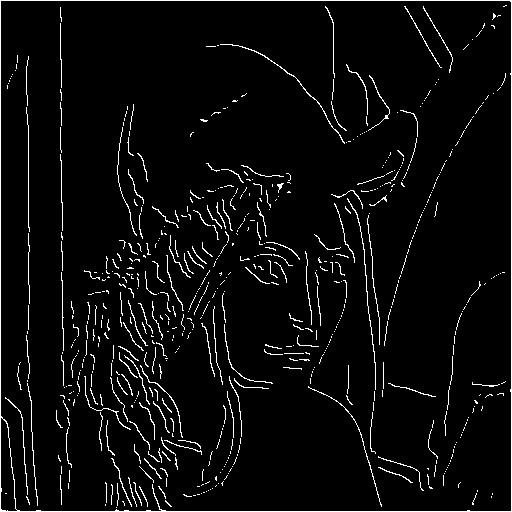
\includegraphics[width=\textwidth]{img/sigma3/lenahys0.png}
\end{subfigure}

\begin{subfigure}{0.33\textwidth}
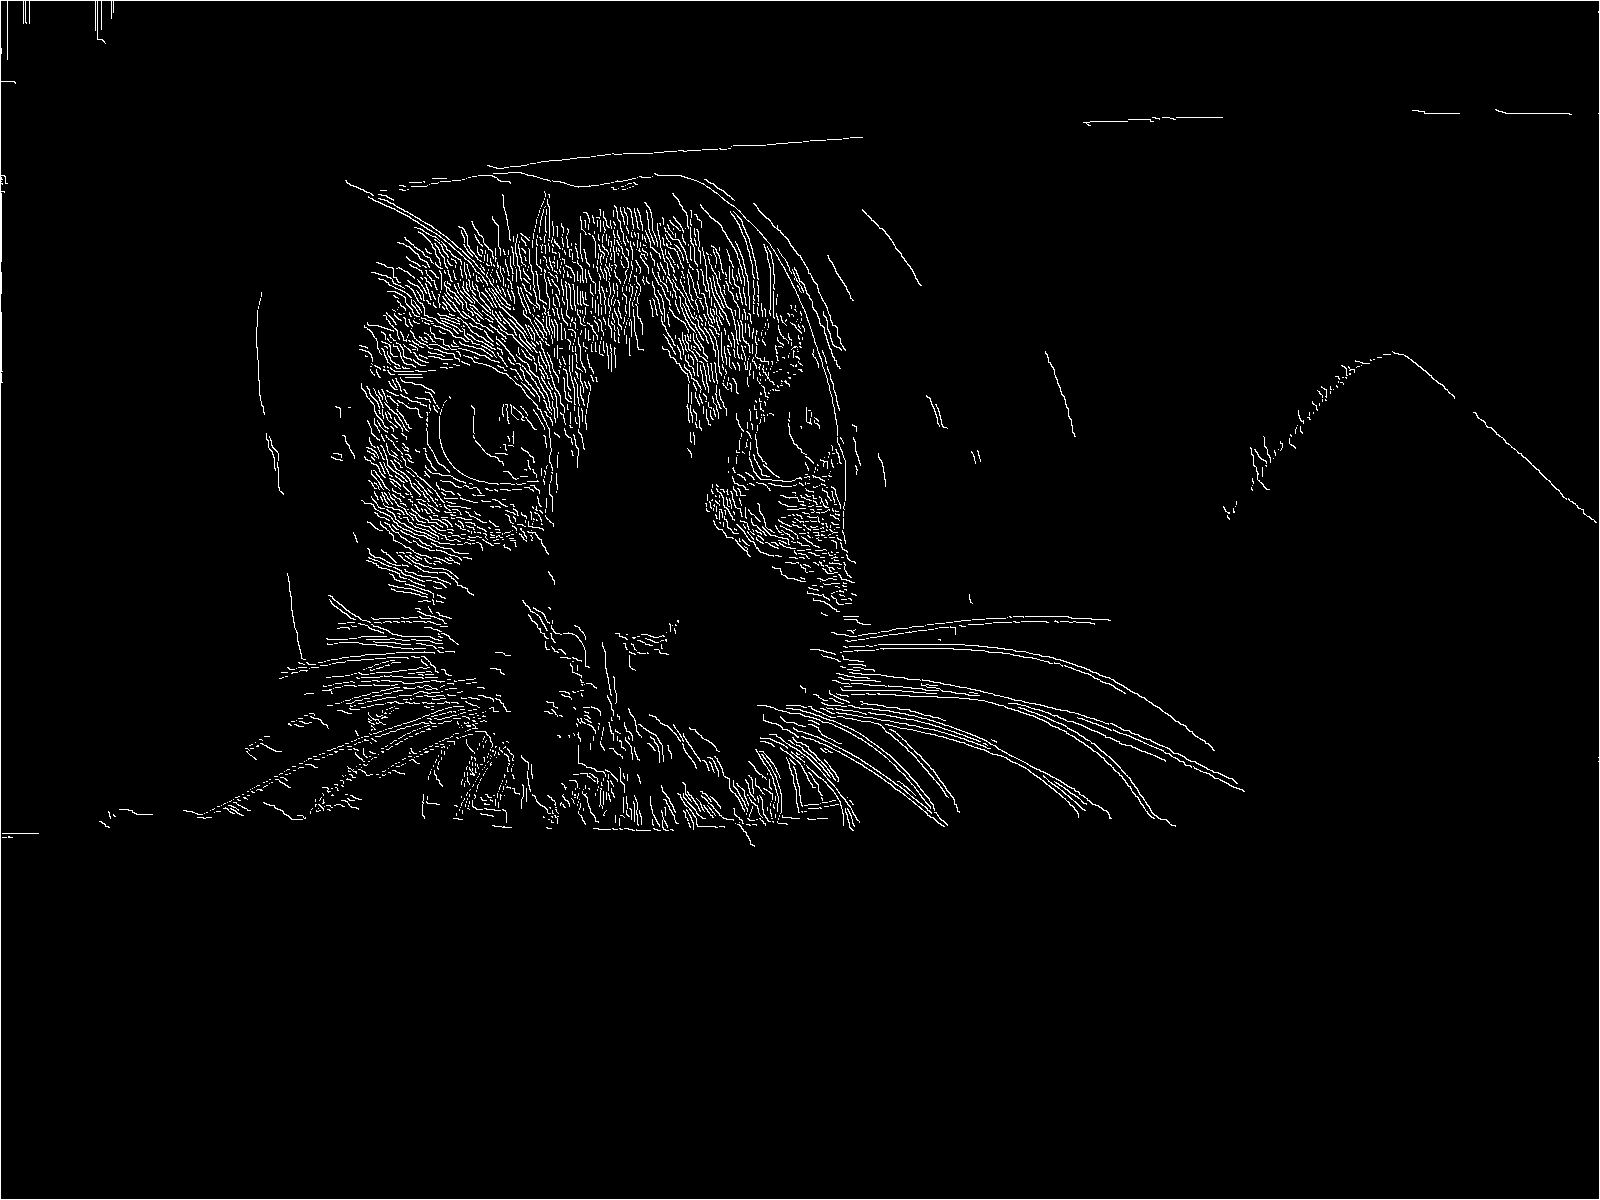
\includegraphics[width=\textwidth]{img/sigma1/cathys0.png}
\end{subfigure}
\begin{subfigure}{0.33\textwidth}
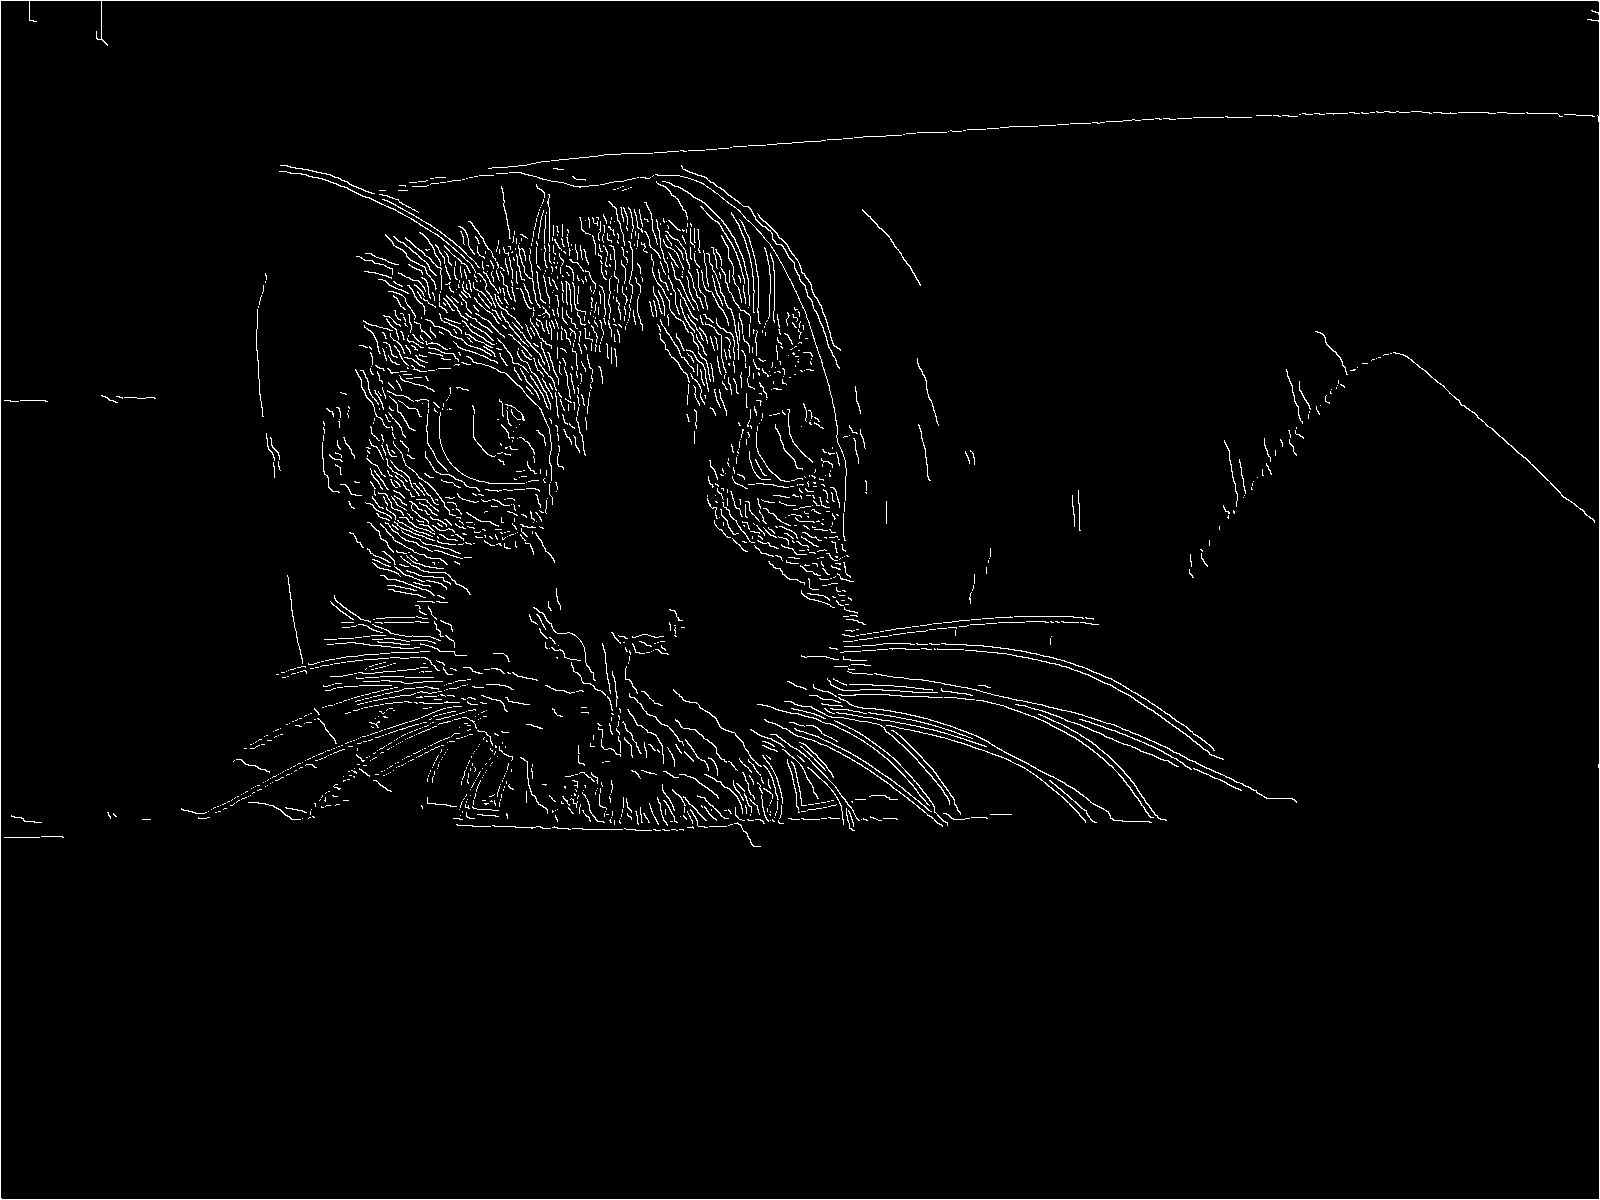
\includegraphics[width=\textwidth]{img/sigma2/cathys0.png}
\end{subfigure}
\begin{subfigure}{0.33\textwidth}
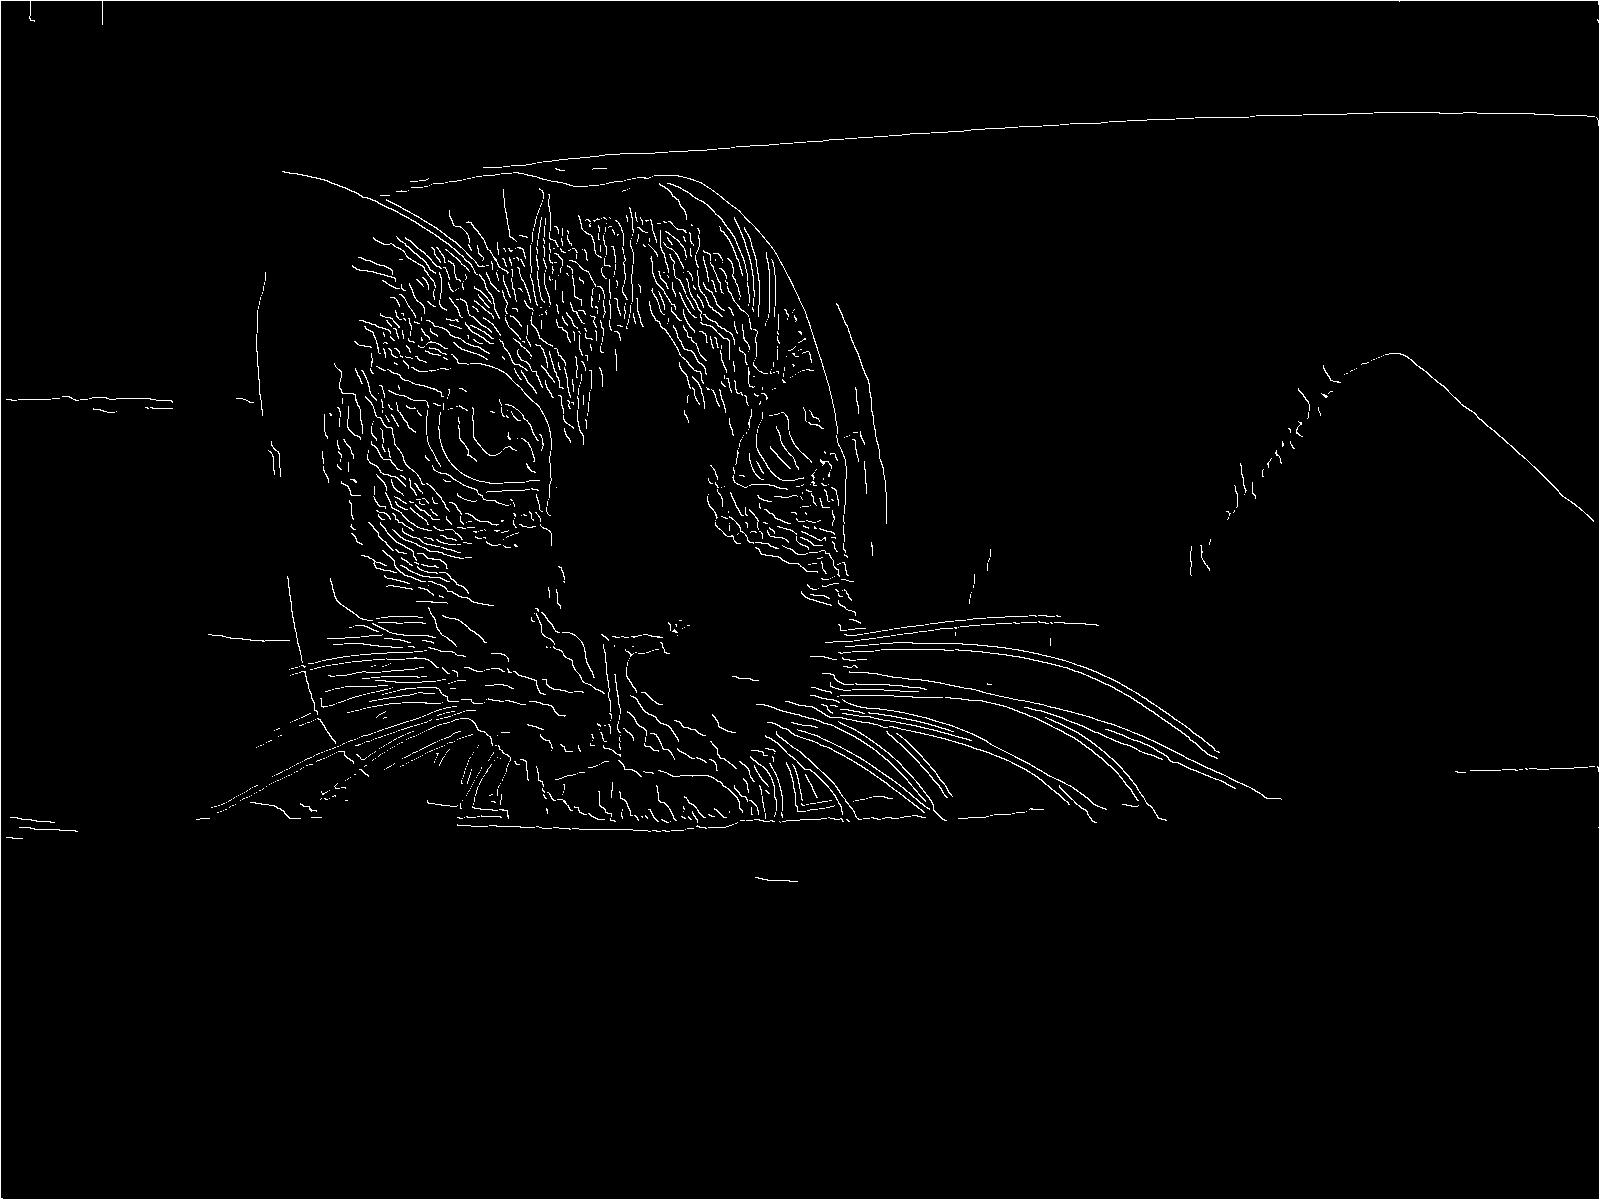
\includegraphics[width=\textwidth]{img/sigma3/cathys0.png}
\end{subfigure}

\caption{Hysteresis thresholding. $\sigma$ = 1, 2 and 3; the high and low thresholds are 0.15 and 0.}

\end{figure}

\end{document}